\documentclass[11pt,a4paper]{article}

% ------------------------------------------------------------------ packages
\usepackage[T1]{fontenc}
\usepackage[utf8]{inputenc}
\usepackage{mathptmx}
\usepackage[scaled=0.9]{helvet}
\usepackage{courier}
\usepackage[a4paper,margin=2.3cm,top=2.4cm,bottom=2.6cm]{geometry}
\usepackage{microtype}
\usepackage{amsmath,amssymb,bm}
\usepackage{graphicx}
\usepackage{booktabs,tabularx,multirow,makecell,colortbl}
\usepackage[table,dvipsnames]{xcolor}
\usepackage{caption,subcaption}
\usepackage{enumitem}
\usepackage{multicol}
\usepackage{float}
\usepackage[section]{placeins}
\renewcommand{\topfraction}{0.9}\renewcommand{\bottomfraction}{0.6}\renewcommand{\textfraction}{0.08}\renewcommand{\floatpagefraction}{0.8}
\setcounter{topnumber}{3}\setcounter{totalnumber}{5}
\usepackage{tikz}
\usetikzlibrary{positioning,arrows.meta,fit,calc,backgrounds,shapes.misc}
\usepackage[most]{tcolorbox}
\usepackage{titlesec}
\usepackage{fancyhdr}
\usepackage[numbers,sort&compress]{natbib}
\usepackage[colorlinks=true,linkcolor=accent,citecolor=accent,urlcolor=accent]{hyperref}
\usepackage[nameinlink,capitalise]{cleveref}
\usepackage{siunitx}
\sisetup{group-separator={,},group-minimum-digits=4}

% ------------------------------------------------------------------ look
\definecolor{accent}{HTML}{1F5FBF}
\definecolor{verified}{HTML}{2A78D6}
\definecolor{reported}{HTML}{8A8A85}
\definecolor{alert}{HTML}{E34948}
\definecolor{ink2}{HTML}{52514E}
\definecolor{panel}{HTML}{F4F6FA}
\definecolor{rule}{HTML}{D9D8D2}

\titleformat{\section}{\sffamily\large\bfseries}{\thesection}{0.7em}{}
\titleformat{\subsection}{\sffamily\normalsize\bfseries}{\thesubsection}{0.6em}{}
\titleformat{\paragraph}[runin]{\sffamily\small\bfseries}{}{}{}[.]
\titlespacing*{\section}{0pt}{2.0ex plus .5ex}{1.0ex}
\titlespacing*{\subsection}{0pt}{1.6ex plus .4ex}{0.6ex}
\captionsetup{font=small,labelfont={sf,bf},labelsep=period,justification=justified,singlelinecheck=false}
\setlength{\parskip}{0.35em}
\setlength{\parindent}{0pt}
\renewcommand{\arraystretch}{1.12}
\setlist{itemsep=0.15em,topsep=0.3em}

\pagestyle{fancy}\fancyhf{}
\renewcommand{\headrulewidth}{0pt}
\fancyfoot[L]{\sffamily\scriptsize\color{ink2}Which provider drew this emoji? \textperiodcentered{} The Winners \textperiodcentered{} IDSI51006}
\fancyfoot[R]{\sffamily\scriptsize\color{ink2}\thepage}

\newcommand{\ver}{\textsuperscript{\textcolor{verified}{\sffamily\scriptsize V}}}
\newcommand{\rep}{\textsuperscript{\textcolor{reported}{\sffamily\scriptsize R}}}
\newcommand{\pct}[1]{#1\%}
\newcommand{\code}[1]{\texttt{#1}}

\newtcolorbox{keybox}[1][]{enhanced,colback=panel,colframe=panel,arc=2pt,boxrule=0pt,left=8pt,right=8pt,top=6pt,bottom=6pt,
  fonttitle=\sffamily\bfseries\small,coltitle=accent,attach title to upper={\par\smallskip},#1}

\hypersetup{pdftitle={Which provider drew this emoji?},pdfauthor={Adam Zeraiki, Lina Oumhand, Charles Montluc-Giannopoulou, Erdem Sanver}}

\begin{document}

% ================================================================== FRONT PAGE
\begin{titlepage}
\thispagestyle{empty}
\vspace*{-0.6cm}
{\sffamily\small\color{accent}\textbf{IDSI51006 COMPUTER VISION} \textperiodcentered{} BSc AIDAMS \textperiodcentered{} ESSEC Business School $\times$ CentraleSup\'elec \textperiodcentered{} Winter 2026}

\vspace{1.4cm}
{\sffamily\fontsize{25}{30}\selectfont\bfseries Which provider drew this emoji?\par}
\vspace{0.35cm}
{\sffamily\Large\color{ink2} Separating drawing style from file-format shortcuts\\ in vendor classification of emoji images\par}

\vspace{0.9cm}
{\large Adam Zeraiki \quad Lina Oumhand \quad Charles Montluc-Giannopoulou \quad Erdem Sanver\par}
\vspace{0.15cm}
{\small\color{ink2} Team \emph{The Winners} \textperiodcentered{} BSc in Artificial Intelligence, Data Analytics and Management Sciences, CentraleSup\'elec and ESSEC Business School\par}
\vspace{0.1cm}
{\small\color{ink2} Course teacher: Titouan Rigaud \textperiodcentered{} 28 October 2026\par}

\vspace{0.9cm}
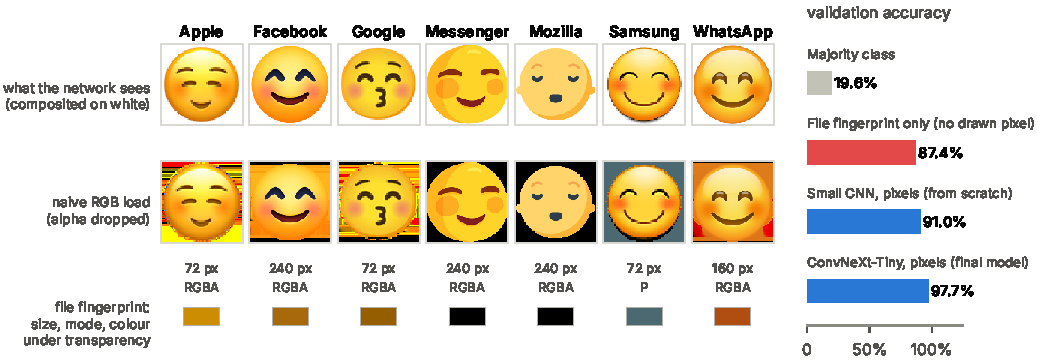
\includegraphics[width=\textwidth]{figs/fig1_teaser.pdf}

\vspace{0.1cm}
\captionof{figure}{\label{fig:teaser}The same kind of emoji as drawn by the seven vendors of the competition. Top: the image every model in this paper receives (alpha-composited on white, upscaled here with nearest-neighbour so that the 72, 160 and 240\,px native resolutions stay visible). Middle: the same files loaded with a naive RGB conversion, which drops the alpha channel and exposes the colour each encoder left under transparent pixels. Bottom: the file fingerprint (native size, PNG mode, mean hidden colour). Right: a random forest on the fingerprint alone, without reading a single drawn pixel, reaches 87.4\% validation accuracy; our final pixel-only network reaches 97.7\%.}

\vfill
\begin{keybox}[title={Result at a glance}]
\small
\begin{tabularx}{\linewidth}{@{}Xr@{}}
Final model: ConvNeXt-Tiny \cite{liu2022convnext}, ImageNet-1k weights, fine-tuned at 224\,px, 5 folds, flip TTA & 27.8\,M parameters\\
Out-of-fold accuracy on all 9{,}879 training images (95\% bootstrap CI) & \textbf{97.69\%} [97.40, 97.98]\\
Kaggle accuracy of the final model, public / private leaderboard & 0.98319 / \textbf{0.98218}\\
Team result: best selected entry, private leaderboard (rank among 18 teams) & 0.98238 (5th)\\
Training cost of the final model on one RTX 4090 & 13 minutes, about \$1\\
\end{tabularx}
\end{keybox}
\end{titlepage}

% ================================================================== SUMMARY, TOC, MODEL CHOSEN
\setcounter{page}{2}
\section*{Abstract}
We classify emoji images by the vendor that drew them (Apple, Facebook, Google, Messenger, Mozilla, Samsung or WhatsApp) on the course's Kaggle competition: \num{9879} labelled training PNGs, \num{9879} test PNGs, accuracy as the metric. Because every vendor draws the same Unicode concepts, this is a \emph{style} recognition problem rather than an object recognition one. Before training any network we audited the files and found that the PNG container leaks the label: native size (72, 160 or 240\,px), Samsung's palette mode and the colour stored under fully transparent pixels let a random forest reach \pct{66.4} from size and mode alone and \pct{87.4} with file statistics, without reading a drawn pixel. We removed this shortcut by design (alpha-compositing on white, one square canvas, exact-pixel augmentation) and measured on a fixed, duplicate-aware split how far the drawing alone can go. A ladder of models climbs from the team's September CNN (\pct{76.7}) to a four-stage BatchNorm CNN trained from scratch (\pct{91.0}) and to ImageNet-pretrained backbones fine-tuned end to end, where input resolution mattered more than architecture. Our final model, ConvNeXt-Tiny fine-tuned at 224\,px in five folds with horizontal-flip test-time augmentation, reaches \pct{97.69} out-of-fold accuracy on all \num{9879} training images and 0.98218 on the private leaderboard. We also report a small but statistically clear finding: keeping the epoch with the lowest validation loss, the usual rule, costs 0.40 points (95\% CI 0.22 to 0.59; exact McNemar $p = 2.4\times10^{-5}$) compared with keeping the last epoch of the OneCycle schedule, because validation loss and accuracy diverge once the network becomes over-confident; \pct{96} of the final model's log loss comes from its \pct{2.3} of errors. The remaining errors stay inside one export family and concentrate on documented look-alikes, such as WhatsApp's 2017 set, which Emojipedia describes as heavily inspired by Apple's. Two side studies complete the picture. A classifier that reads only the PNG bytes reaches \pct{93.5}, so the shortcut could not have taken us to 99\%; as a third expert next to DINOv2 and ConvNeXt it adds up to 0.9 points on held-out images, while a hosted decision model (Jev) asked to arbitrate between the experts did worse than a plain average. And a replication of the double-descent protocol of Nakkiran et al.\ (ResNet18 from scratch, 11 widths, up to 4{,}000 epochs) shows the epoch-wise second descent on our data only when labels are deliberately corrupted, consistent with its absence from our real training curves.

\vspace{0.4em}
\begin{keybox}[title={Model chosen}]
\small
\textbf{Type: a convolutional neural network.} The final model is \textbf{ConvNeXt-Tiny} \cite{liu2022convnext} (27.8\,M parameters), initialised from ImageNet-1k weights \cite{deng2009imagenet,wightman2019timm} and fully fine-tuned on $224\times224$ inputs; five fold-models are averaged with horizontal-flip test-time augmentation. A 0.39\,M-parameter CNN trained from scratch (EmojiCNNv2) serves as the reference for ablations and explainability.

\textbf{Why not a vision-language model.} All seven classes contain the same objects; the signal is how they are drawn (outlines, shading, anti-aliasing), which early convolutional filters capture \cite{gatys2016style} and which a model trained to describe image \emph{content} is not built for. A CNN also trains in minutes, can be inspected (Grad-CAM, confusion structure) and reproduced exactly.

\textbf{Why not hand-crafted features or frozen features.} Colour histograms with HOG and an SVM reached \pct{81.3}\rep, below every CNN; ResNet18 used as a frozen feature extractor with a linear head reached \pct{77.5}\rep{} and \pct{93.7}\rep{} once fine-tuned. Frozen features became competitive only with hand-crafted style descriptors and an RBF-kernel SVM on top (\pct{96.8}\rep). Style lives below the object-level features that ImageNet training rewards; the backbone must be adapted.
\end{keybox}

{\small\color{ink2}\textbf{Notation.} Numbers marked \ver{} or untagged were produced by the submitted codebase and can be recomputed from its saved outputs; numbers marked \rep{} come from Erdem's experiment log (13 to 14 October, \cref{app:log}) or from Kaggle entries that the codebase does not reproduce.\par}

\clearpage
{\small\renewcommand{\contentsname}{\large Contents}\begin{multicols}{2}\tableofcontents\end{multicols}}
\vspace{0.6em}

% ================================================================== 1 INTRODUCTION
\section{Introduction}
\label{sec:intro}

Every major platform ships its own drawing of the same Unicode emoji. A grinning face is a grinning face on every phone, yet an attentive reader can usually tell an Apple face from a Samsung one: the gradients, the outline weight, the shape of the eyes and the palette are a vendor's signature. The course challenge asks a model to do the same from a single PNG. This makes it a cousin of style recognition \cite{karayev2014style} and font identification \cite{wang2015deepfont}, where the classes share content and differ in rendering, rather than of object recognition, where content is the class.

Such tasks are prone to shortcut learning \cite{geirhos2020shortcut}: a network rewarded only for accuracy will exploit any cue that correlates with the label, including cues that have nothing to do with the drawing. In this dataset the cue is the file itself. Each vendor exported its set through its own pipeline, and the pipeline left fingerprints in the container (\cref{sec:fingerprints}). A related risk is leakage through duplicates \cite{kaufman2012leakage,barz2020cifair}: the competition data contain exact copies within the training set and across training and test. Both issues decide whether a validation number measures what we think it measures, so we treat them before modelling.

\paragraph{Contributions}
\begin{enumerate}[leftmargin=1.4em]
  \item A file-level audit that quantifies the container shortcut: \pct{87.4} accuracy without any drawn pixel, and a preprocessing recipe that removes it while keeping the rendering intact (\cref{sec:data}).
  \item A controlled ladder of models on a fixed, duplicate-aware split, from the team's first CNN to a fine-tuned ConvNeXt-Tiny, with every verified number recomputable from saved probabilities (\cref{sec:ladder}).
  \item A final model at \pct{97.69} out-of-fold accuracy and 0.98218 private leaderboard accuracy, trained in 13 minutes on one consumer GPU (\cref{sec:final}).
  \item Evidence that, at this accuracy, the rule used to pick a checkpoint matters: keeping the last epoch beats keeping the lowest-validation-loss epoch by 0.40 points, explained by over-confidence on a few hard images (\cref{sec:epoch}).
  \item A look at the non-monotonic validation curves through the lens of double descent, and a fitting diagnosis: the first CNN underfitted, the final model fits its training set but overfits only in its confidence, not its decisions (\cref{sec:descent,sec:fit}).
  \item An error analysis showing that the model separates export families from pixels alone and fails on documented look-alike designs (\cref{sec:errors}).
\end{enumerate}

\paragraph{Outline} \Cref{sec:background} introduces the families of models we used, from random forests to vision transformers. \Cref{sec:data} describes the data and the preprocessing, \cref{sec:arch} the architectures, \cref{sec:metrics} the metrics and \cref{sec:perf} the results, starting with the path from our first model to the final one (\cref{sec:journey}). \Cref{sec:code} covers the code and the use of AI, and \cref{sec:conclusion} concludes.

% ================================================================== 2 BACKGROUND
\section{Background: the model families we used}
\label{sec:background}
The project moved through most of the families of models used in computer vision today, from hand-crafted features to self-supervised transformers. This section introduces each one at the level needed to follow the rest of the paper; \cref{tab:families} summarises them and points to where each appears in our experiments.

\begin{table}[t]
\centering\small
\caption{\textbf{Model families at a glance}, with the best validation (or private leaderboard, $^\dagger$) accuracy each reached in this project. Parameter counts are for the seven-class versions, counted with \texttt{timm}.}
\label{tab:families}
\begin{tabularx}{\textwidth}{@{}>{\raggedright\arraybackslash}p{30mm}>{\raggedright\arraybackslash}X>{\raggedright\arraybackslash}X>{\raggedleft\arraybackslash}p{15mm}>{\raggedleft\arraybackslash}p{15mm}@{}}
\toprule
Family & What it sees & Built-in assumption & Params & Best here\\
\midrule
Random forest, SVM & hand-made features (file statistics, colour histogram, HOG) & the features are the right ones & n/a & 87.37\%\\
CNN from scratch & pixels, through small local filters & locality, translation equivariance & 0.39\,M & 90.96\%\\
Pretrained CNN (ResNet18, EfficientNet-B0, ConvNeXt-Tiny) & pixels, filters initialised on ImageNet & as above, plus ImageNet features transfer & 4.0--27.8\,M & 97.69\%\\
Vision transformer (DINOv2) & $14\times14$ patches as tokens, global attention & almost none; learned from 142\,M images & 22.1\,M (S/14) & 0.95607$^\dagger$\\
Ensembles and fusion & the outputs of several models & errors of the members are not identical & sum & 0.98238$^\dagger$\\
\bottomrule
\end{tabularx}
\end{table}

\subsection{Classical machine learning on hand-crafted features}
Before deep learning, an image classifier had two separate parts: a human-designed feature extractor and a generic classifier. Histograms of oriented gradients (HOG) \cite{dalal2005hog} describe local shape by the distribution of edge directions in small cells; colour histograms describe the palette. A support vector machine \cite{cortes1995svm} then finds the maximum-margin boundary between classes, possibly in a higher-dimensional space reached through a kernel, and a random forest \cite{breiman2001rf} averages many decision trees, each trained on a bootstrap sample with random feature subsets. Both are fast and interpretable, but they can only use the information the features expose. We used them three times: as a diagnostic of the file-format shortcut (a random forest on file metadata, \cref{sec:fingerprints}) as hand-crafted baselines on pixels (HOG and colour histogram with an SVM, \pct{81.28}; extra-trees on pixels, colour and transparency, \pct{82.14}), and on top of frozen ResNet18 features, where an RBF-kernel SVM reached \pct{96.76} (\cref{sec:arch}).

\subsection{Convolutional neural networks}
A convolutional neural network (CNN) \cite{lecun1998gradient,krizhevsky2012alexnet} learns the features instead. A convolutional layer slides a small filter $w$ of size $k\times k$ over the input and computes, at every position and for every output channel $c'$,
\begin{equation}
  y_{c'}(i,j) \;=\; b_{c'} + \sum_{c}\sum_{u,v=-\lfloor k/2\rfloor}^{\lfloor k/2\rfloor} w_{c',c}(u,v)\, x_c(i+u,\, j+v),
\end{equation}
so the same few weights are reused across the image (\cref{fig:cnn-basics}). Two assumptions are built in: what matters is local (locality), and a pattern means the same thing wherever it appears (translation equivariance). Pooling layers downsample the feature maps, so each later filter sees a larger part of the image (its receptive field), and stacking layers builds a hierarchy from edges to textures to parts. Batch normalisation \cite{ioffe2015batchnorm} standardises activations within each mini-batch and makes deeper networks trainable at larger learning rates. These biases suit our task well: anti-aliasing, outline weight and shading are local, repeated patterns.

\begin{figure}[t]
\centering
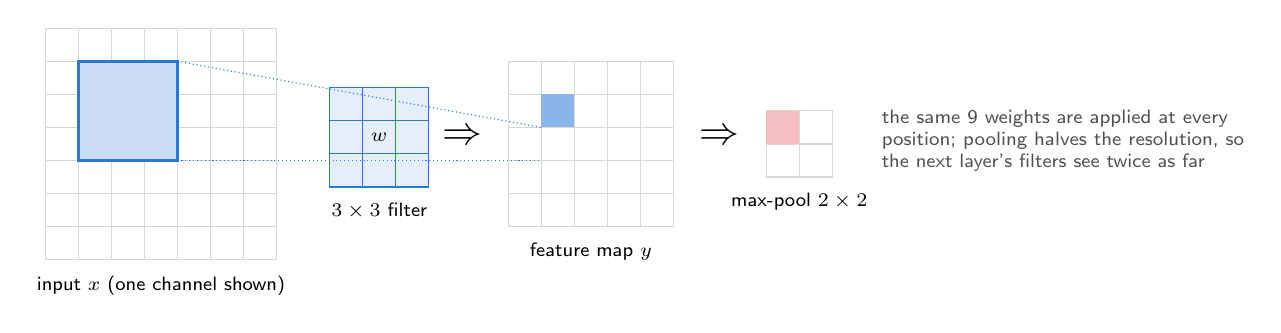
\begin{tikzpicture}[font=\sffamily\scriptsize, x=4.2mm, y=4.2mm,
  arr/.style={-{Stealth[length=2mm]}, color=ink2, line width=0.6pt}]
  % input grid 7x7
  \foreach \i in {0,...,6} \foreach \j in {0,...,6} \draw[rule, fill=white] (\i,\j) rectangle ++(1,1);
  \fill[verified!25] (1,3) rectangle (4,6); \draw[verified, line width=0.9pt] (1,3) rectangle (4,6);
  \node[anchor=north] at (3.5,-0.2) {input $x$ (one channel shown)};
  % kernel
  \begin{scope}[shift={(8.6,2.2)}]
    \foreach \i in {0,...,2} \foreach \j in {0,...,2} \draw[verified, fill=verified!12] (\i,\j) rectangle ++(1,1);
    \node at (1.5,1.5) {$w$};
    \node[anchor=north] at (1.5,-0.2) {$3\times3$ filter};
  \end{scope}
  \node at (12.6,3.7) {\Large$\Rightarrow$};
  % feature map 5x5
  \begin{scope}[shift={(14,1)}]
    \foreach \i in {0,...,4} \foreach \j in {0,...,4} \draw[rule, fill=white] (\i,\j) rectangle ++(1,1);
    \fill[verified!55] (1,3) rectangle (2,4);
    \node[anchor=north] at (2.5,-0.2) {feature map $y$};
  \end{scope}
  \draw[densely dotted, verified] (4,6) -- (15,4); \draw[densely dotted, verified] (4,3) -- (15,3);
  \node at (20.4,3.7) {\Large$\Rightarrow$};
  % pooled 2x2 (from 4x4 top-left region)
  \begin{scope}[shift={(21.8,2.5)}]
    \foreach \i in {0,...,1} \foreach \j in {0,...,1} \draw[rule, fill=white] (\i,\j) rectangle ++(1,1);
    \fill[alert!35] (0,1) rectangle (1,2);
    \node[anchor=north, align=center] at (1,-0.2) {max-pool $2\times2$};
  \end{scope}
  \node[align=left, anchor=west, text width=46mm, color=ink2] at (25,3.6) {the same 9 weights are applied at every position; pooling halves the resolution, so the next layer's filters see twice as far};
\end{tikzpicture}
\caption{\textbf{What a convolutional layer computes.} A $3\times3$ filter (blue) slides over the input and produces one value of the feature map per position; max-pooling then keeps the strongest response in each $2\times2$ window.}
\label{fig:cnn-basics}
\end{figure}

\subsection{Deeper CNNs: residual, efficient and modernised blocks}
Simply stacking more layers eventually makes networks harder to optimise. ResNet \cite{he2016resnet} adds the input of each block to its output, $\bm{x}\leftarrow\bm{x}+F(\bm{x})$, so that a block only has to learn a correction and gradients flow through the identity path; ResNet18 stacks eight such blocks of two $3\times3$ convolutions. EfficientNet-B0 \cite{tan2019efficientnet} is built from the inverted bottleneck (MBConv) of MobileNetV2 \cite{sandler2018mobilenetv2}: a $1\times1$ convolution expands the channels, a cheap depthwise $3\times3$ convolution filters each channel separately, a squeeze-and-excitation gate \cite{hu2018senet} reweights channels, and a $1\times1$ convolution projects back. ConvNeXt \cite{liu2022convnext} revisits ResNet with design choices borrowed from transformers: a $7\times7$ depthwise convolution, LayerNorm instead of BatchNorm, a four-times expansion, GELU and fewer normalisation layers. \Cref{fig:blocks} compares the three blocks; ConvNeXt-Tiny became our final backbone.

\begin{figure}[t]
\centering
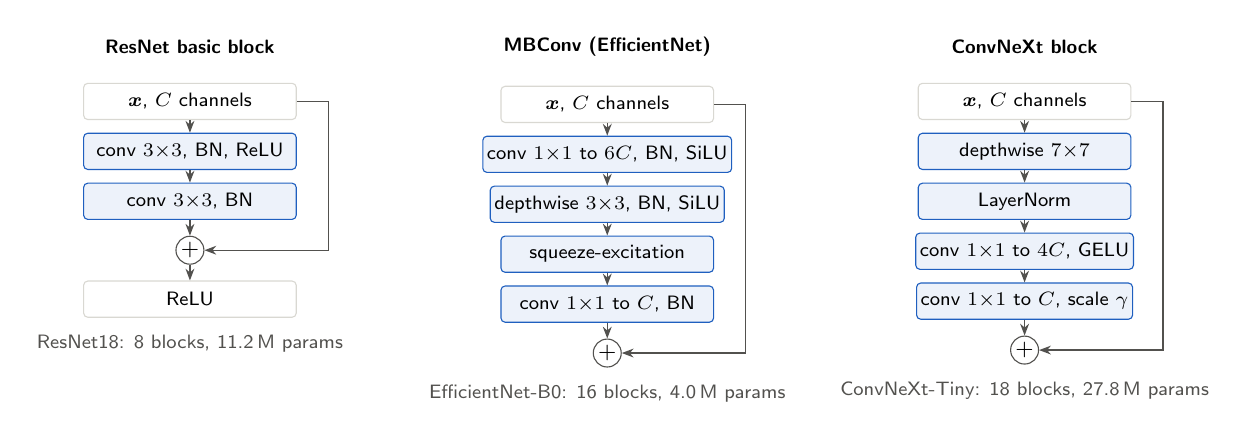
\begin{tikzpicture}[font=\sffamily\scriptsize, node distance=1.6mm,
  l/.style={draw=accent, rounded corners=1.5pt, fill=accent!8, minimum width=27mm, minimum height=4.6mm, inner sep=1.5pt, align=center},
  n/.style={draw=rule, rounded corners=1.5pt, fill=white, minimum width=27mm, minimum height=4.6mm, inner sep=1.5pt, align=center},
  arr/.style={-{Stealth[length=1.5mm]}, color=ink2, line width=0.5pt},
  plus/.style={circle, draw=ink2, inner sep=0.5pt, font=\sffamily\footnotesize}]
  % ResNet basic block
  \node[font=\sffamily\scriptsize\bfseries] (t1) at (0,0) {ResNet basic block};
  \node[n, below=2.5mm of t1] (a0) {$\bm{x}$, $C$ channels};
  \node[l, below=of a0] (a1) {conv $3{\times}3$, BN, ReLU};
  \node[l, below=of a1] (a2) {conv $3{\times}3$, BN};
  \node[plus, below=2mm of a2] (ap) {$+$};
  \node[n, below=2mm of ap] (a3) {ReLU};
  \foreach \u/\v in {a0/a1,a1/a2,a2/ap,ap/a3} \draw[arr] (\u) -- (\v);
  \draw[arr] (a0.east) -- ++(4mm,0) |- (ap.east);
  \node[color=ink2, below=1mm of a3, align=center] {ResNet18: 8 blocks, 11.2\,M params};
  % MBConv
  \node[font=\sffamily\scriptsize\bfseries] (t2) at (5.3,0) {MBConv (EfficientNet)};
  \node[n, below=2.5mm of t2] (b0) {$\bm{x}$, $C$ channels};
  \node[l, below=of b0] (b1) {conv $1{\times}1$ to $6C$, BN, SiLU};
  \node[l, below=of b1] (b2) {depthwise $3{\times}3$, BN, SiLU};
  \node[l, below=of b2] (b3) {squeeze-excitation};
  \node[l, below=of b3] (b4) {conv $1{\times}1$ to $C$, BN};
  \node[plus, below=2mm of b4] (bp) {$+$};
  \foreach \u/\v in {b0/b1,b1/b2,b2/b3,b3/b4,b4/bp} \draw[arr] (\u) -- (\v);
  \draw[arr] (b0.east) -- ++(4mm,0) |- (bp.east);
  \node[color=ink2, below=1mm of bp, align=center] {EfficientNet-B0: 16 blocks, 4.0\,M params};
  % ConvNeXt block
  \node[font=\sffamily\scriptsize\bfseries] (t3) at (10.6,0) {ConvNeXt block};
  \node[n, below=2.5mm of t3] (c0) {$\bm{x}$, $C$ channels};
  \node[l, below=of c0] (c1) {depthwise $7{\times}7$};
  \node[l, below=of c1] (c2) {LayerNorm};
  \node[l, below=of c2] (c3) {conv $1{\times}1$ to $4C$, GELU};
  \node[l, below=of c3] (c4) {conv $1{\times}1$ to $C$, scale $\gamma$};
  \node[plus, below=2mm of c4] (cp) {$+$};
  \foreach \u/\v in {c0/c1,c1/c2,c2/c3,c3/c4,c4/cp} \draw[arr] (\u) -- (\v);
  \draw[arr] (c0.east) -- ++(4mm,0) |- (cp.east);
  \node[color=ink2, below=1mm of cp, align=center] {ConvNeXt-Tiny: 18 blocks, 27.8\,M params};
\end{tikzpicture}
\caption{\textbf{The three convolutional blocks we fine-tuned.} All three add a learned correction to their input (the arrow on the right is the residual connection). They differ in how they filter: two dense $3\times3$ convolutions (ResNet), an expand, depthwise-filter and project sequence with channel gating (MBConv), or one large $7\times7$ depthwise filter followed by a transformer-style MLP (ConvNeXt).}
\label{fig:blocks}
\end{figure}

\subsection{Transformers and the Vision Transformer}
The transformer \cite{vaswani2017attention} processes a sequence of tokens with self-attention: every token is projected to a query $q$, a key $k$ and a value $v$, and each output is a weighted average of all values, with weights given by query-key similarity,
\begin{equation}
  \operatorname{Attention}(Q,K,V)=\operatorname{softmax}\!\Big(\frac{QK^\top}{\sqrt{d}}\Big)V .
\end{equation}
The Vision Transformer (ViT) \cite{dosovitskiy2021vit} applies this to images by cutting them into fixed-size patches, embedding each patch as a token, adding a position embedding and a learnable class token, and passing the sequence through a stack of attention and MLP layers (\cref{fig:vit}). Unlike a CNN, a ViT assumes almost nothing about images: any patch can attend to any other from the first layer, and locality must be learned from data. This makes ViTs data-hungry, which is why they are almost always used after large-scale pretraining.

\begin{figure}[t]
\centering
\begin{tikzpicture}[font=\sffamily\scriptsize, x=1mm, y=1mm,
  arr/.style={-{Stealth[length=1.8mm]}, color=ink2, line width=0.6pt},
  tok/.style={draw=accent, fill=accent!15, minimum width=4.2mm, minimum height=5.5mm, inner sep=0pt},
  box/.style={draw=accent, rounded corners=2pt, fill=accent!6, align=center, inner sep=3pt}]
  % image with patch grid
  \node[anchor=south west, inner sep=0] (img) at (0,0) {
\includegraphics[width=22mm]{figs/vit_input.png}};
  \foreach \k in {1,...,3} { \draw[white, line width=0.8pt] (\k*5.5,0) -- (\k*5.5,22); \draw[white, line width=0.8pt] (0,\k*5.5) -- (22,\k*5.5); }
  \node[anchor=north, align=center] at (11,-1) {image cut into patches\\($16\times16$ grid of $14\,$px at 224\,px)};
  % tokens
  \draw[arr] (24,11) -- (30,11);
  \node[tok, fill=alert!25, draw=alert] (cls) at (34,11) {};
  \node[above=0.3mm of cls, color=alert] {\textsc{cls}};
  \foreach \t in {1,...,6} \node[tok] at (34+\t*5,11) {};
  \node at (69,11) {$\cdots$};
  \node[anchor=north, align=center] at (52,5) {linear embedding of each patch\\+ position embedding};
  % encoder
  \draw[arr] (75,11) -- (80,11);
  \node[box, anchor=west, minimum height=21mm, text width=29mm] (enc) at (80,11) {\textbf{transformer encoder}\\[2pt] LayerNorm $\to$ multi-head self-attention $\to$ $+$\\[2pt] LayerNorm $\to$ MLP $\to$ $+$\\[2pt] {\color{ink2}repeated 12 times (ViT-S/B)}};
  \draw[arr] (enc.east) -- ++(5,0) node[right, box, fill=white, draw=rule] {\textsc{cls} token\\$\to$ linear $\to$ 7};
\end{tikzpicture}
\caption{\textbf{Vision Transformer.} The image becomes a sequence of patch tokens; self-attention lets every patch interact with every other one in every layer, and the class token's final state is used for classification. DINOv2 models use 14-pixel patches.}
\label{fig:vit}
\end{figure}

\subsection{Pretraining and transfer learning}
Training a large network from scratch on \num{9879} images would overfit. Transfer learning starts instead from weights learned on a much larger dataset and adapts them. With \emph{supervised} pretraining, the network was trained to classify ImageNet's 1.28 million photographs into 1{,}000 classes \cite{deng2009imagenet}; all our pretrained CNNs come from this setting. With \emph{self-supervised} pretraining, no labels are used at all: DINO \cite{caron2021dino} trains a student network to match the output of a teacher network, an exponential moving average of the student, on different augmented crops of the same image, and DINOv2 \cite{oquab2024dinov2} scales this recipe to 142 million curated images. Either way, the pretrained network can be used \emph{frozen}, as a fixed feature extractor with only a new linear head trained, or \emph{fine-tuned}, with every weight updated at a small learning rate. Which of the two works depends on how close the pretraining task is to the new one; for vendor style, it turned out to be far (\cref{sec:journey}).

\subsection{Combining models}
An ensemble averages the predictions of several models; it helps when their errors differ \cite{dietterich1998tests,lakshminarayanan2017ensembles}. Soft voting averages probabilities with equal weights. Stacking \cite{wolpert1992stacking} trains a second-level model on the first-level models' predictions, which must be made on data those models did not train on (out-of-fold predictions), otherwise the meta-model learns to trust overfitted members. A learned fusion goes one step further and combines the members' internal features rather than their final probabilities; we describe our version in \cref{sec:fusion}.


% ================================================================== 2 DATA AND PREPROCESSING
\section{Data and preprocessing}
\label{sec:data}

\subsection{The dataset}
The archive contains \num{9879} training PNGs with labels and \num{9879} unlabelled test PNGs. Classes are imbalanced (\cref{fig:dataset}a): Apple has \num{1924} images, Google \num{1877}, Samsung \num{1790}, Facebook \num{1667} and WhatsApp \num{1644}, while Messenger has 580 (\pct{5.9}) and Mozilla 397 (\pct{4.0}). Predicting the majority class gives \pct{19.5}; chance is \pct{14.3}.

\begin{figure}[t]
  \centering
  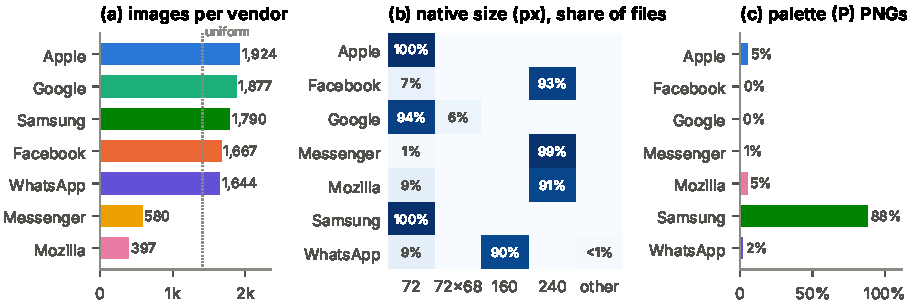
\includegraphics[width=\textwidth]{figs/fig2_dataset.pdf}
  \caption{\textbf{The training set and its file formats.} (a) Images per vendor; the dotted line is a uniform split. (b) Native PNG size as a share of each vendor's files: three export families (72\,px, 160\,px, 240\,px) almost coincide with groups of vendors. (c) Share of palette-mode PNGs: Samsung is the only vendor that saves most files as palette (P) images.}
  \label{fig:dataset}
\end{figure}

\subsection{What the files reveal before any pixel is read}
\label{sec:fingerprints}
\Cref{tab:fingerprints} and \cref{fig:dataset,fig:hidden} summarise what the containers say. Apple, Google and Samsung files are 72\,px wide, WhatsApp files 160\,px, and Facebook, Messenger and Mozilla files 240\,px. Samsung saved \pct{88} of its files as palette PNGs, where every other vendor used RGBA. The RGB values stored under fully transparent pixels, invisible on any screen, differ by vendor too, because an encoder keeps whatever was in its buffer (\cref{fig:hidden}a): near-black for Mozilla, one near-constant blue-grey for Samsung, a brownish mixture elsewhere. Messenger and Facebook share the 240\,px export because Facebook replaced the Messenger-specific set with its platform-wide set in October 2017 \cite{emojipedia2017messenger}. The test set has the same mix: the total variation distance between the train and test distributions of size and mode is \pct{0.5}.

\begin{table}[t]
\centering\small
\caption{\textbf{File-level fingerprints per vendor}, computed on the real training files\ver. The hidden colour is the mean RGB under fully transparent pixels, averaged over the vendor's files.}
\label{tab:fingerprints}
\begin{tabular}{@{}lrllcr@{}}
\toprule
Vendor & Images & Modal size (share) & Modal mode (share) & Hidden colour (R, G, B) & Transparent\\
\midrule
Apple     & \num{1924} & $72\times72$ (99.9\%)   & RGBA (93.9\%) & 46.7, 39.1, 29.8 & 40\%\\
Facebook  & \num{1667} & $240\times240$ (93.0\%) & RGBA (99.0\%) & 85.0, 68.1, 56.0 & 42\%\\
Google    & \num{1877} & $72\times72$ (93.6\%)   & RGBA (98.0\%) & 26.3, 21.9, 17.9 & 40\%\\
Messenger & 580        & $240\times240$ (98.6\%) & RGBA (99.5\%) & 33.8, 29.4, 24.8 & 42\%\\
Mozilla   & 397        & $240\times240$ (91.2\%) & RGBA (95.2\%) & 5.5, 5.6, 5.5    & 37\%\\
Samsung   & \num{1790} & $72\times72$ (99.7\%)   & P (88.3\%)    & 70.6, 96.0, 98.7 & 46\%\\
WhatsApp  & \num{1644} & $160\times160$ (90.3\%) & RGBA (96.9\%) & 68.7, 54.7, 44.3 & 47\%\\
\bottomrule
\end{tabular}
\end{table}

We then measured how much these fingerprints are worth (\cref{fig:hidden}b). Classifiers that never see a drawn pixel reach \pct{64.6} (logistic regression) and \pct{66.4} (random forest) from width, height, PNG mode and the alpha flag, \pct{84.4} once file size and transparent fraction are added, and \pct{87.4} with the hidden colour\ver. A network given the raw file would be free to learn this instead of the drawing, and its validation score would look excellent for the wrong reason. We therefore removed the shortcut (\cref{sec:recipe}) and kept the metadata out of the final model; \cref{sec:ladder} measures, as an ablation, what it would have added on top of pixels.

\begin{figure}[t]
  \centering
  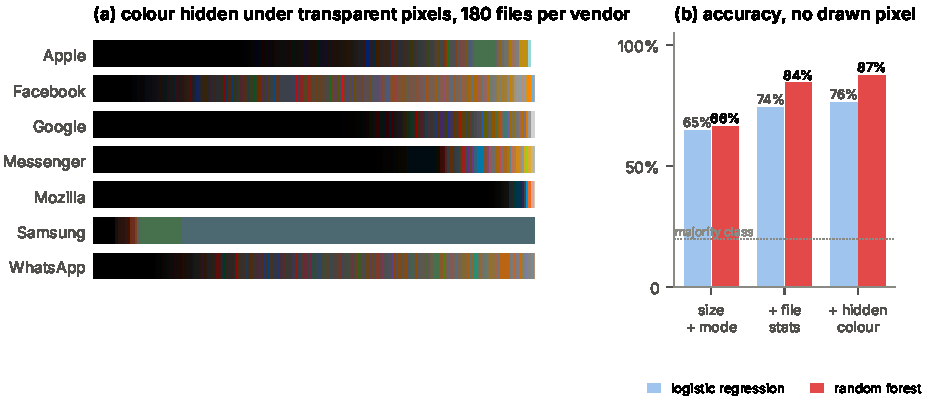
\includegraphics[width=\textwidth]{figs/fig3_hidden_colour.pdf}
  \caption{\textbf{The container leaks the label.} (a) Each strip shows the mean colour stored under fully transparent pixels for 180 random files of a vendor, sorted by luminance; these pixels are invisible when the image is displayed. Samsung's palette files share one blue-grey, Mozilla's are black. (b) Validation accuracy of models that see only file metadata (stored split, \num{1979} images)\ver: up to \pct{87.4} without a single drawn pixel.}
  \label{fig:hidden}
\end{figure}

\subsection{Preprocessing recipe}
\label{sec:recipe}
One function feeds every model in this paper. Let $F\in[0,255]^{H\times W\times3}$ be the stored colour and $\alpha\in[0,1]^{H\times W}$ the alpha channel of a file. We compute
\begin{equation}
  I \;=\; \alpha\odot F + (1-\alpha)\odot 255 ,
\end{equation}
which sets every transparent pixel to white and therefore erases the hidden colour (\cref{fig:teaser}, \cref{fig:pipeline}). The image is then fitted into a square canvas keeping its aspect ratio (Lanczos filter) and padded with white, because a few Google files are $72\times68$; resized to the model's input (96\,px for networks trained from scratch, 224\,px for ConvNeXt-Tiny); stored as \texttt{uint8} and cached; and normalised to $[-1,1]$ for networks trained from scratch or with the ImageNet mean and standard deviation for the pretrained backbone. We do not crop, do not convert to greyscale (palettes are part of a vendor's style) and do not equalise histograms. Resizing to a common canvas also removes the native size as a direct cue; whatever the network learns about it must come from the rendering.

The team measured the effect of compositing directly: the same three-block CNN scored \pct{92.11} with a default RGB load and \pct{93.62} with alpha compositing on white, everything else equal (E2 and E3\rep). The naive load also exposes the hidden colour, so the composited input wins even though it gives the network less to cheat with. The resampling filter matters for the same reason: E15, the team's best Kaggle entry, adds models trained at 144 and 216\,px with nearest-neighbour resizing, which are exact $2\times$ and $3\times$ copies of a 72\,px file with no interpolated pixel (\cref{sec:kaggle}).

\begin{figure}[t]
  \centering
  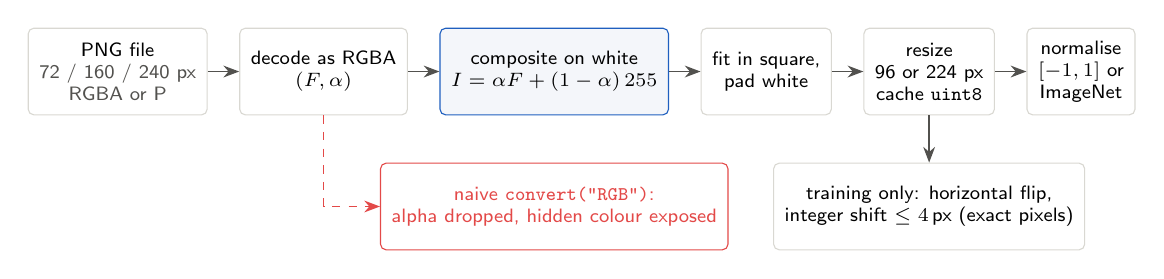
\begin{tikzpicture}[font=\sffamily\scriptsize, node distance=4mm,
    box/.style={draw=rule, fill=white, rounded corners=2pt, align=center, inner sep=4pt, minimum height=11mm},
    hl/.style={box, draw=accent, fill=panel},
    arr/.style={-{Stealth[length=2mm]}, color=ink2, line width=0.6pt}]
    \node[box] (png) {PNG file\\{\color{ink2}72 / 160 / 240 px}\\{\color{ink2}RGBA or P}};
    \node[box, right=of png] (rgba) {decode as RGBA\\$(F,\alpha)$};
    \node[hl, right=of rgba] (comp) {composite on white\\$I=\alpha F+(1-\alpha)\,255$};
    \node[box, right=of comp] (fit) {fit in square,\\pad white};
    \node[box, right=of fit] (res) {resize\\96 or 224 px\\cache \texttt{uint8}};
    \node[box, right=of res] (norm) {normalise\\$[-1,1]$ or\\ImageNet};
    \foreach \a/\b in {png/rgba,rgba/comp,comp/fit,fit/res,res/norm} \draw[arr] (\a) -- (\b);
    \node[box, below=6mm of comp, draw=alert, text=alert] (bad) {naive \texttt{convert("RGB")}:\\alpha dropped, hidden colour exposed};
    \draw[arr, color=alert, dashed] (rgba.south) |- (bad.west);
    \node[box, below=6mm of res, minimum width=36mm] (aug) {training only: horizontal flip,\\integer shift $\le 4$\,px (exact pixels)};
    \draw[arr] (res.south) -- (aug.north);
  \end{tikzpicture}
  \caption{\textbf{Preprocessing pipeline} shared by every model. Compositing on white is the step that removes the hidden-colour shortcut of \cref{fig:hidden}; the naive branch (red) is what a default RGB load does.}
  \label{fig:pipeline}
\end{figure}

\subsection{Data augmentation}
Training augmentation is limited to a horizontal flip and an integer translation of up to 4\,px (white padding, random crop). Both are exact pixel operations: no interpolation touches the image, so the anti-aliased outlines and gradients that distinguish vendors stay exactly as exported. Rotation and rescaling resample the image and blur precisely that signal. The team tested it: on ConvNeXt-Tiny at 128\,px, rotation and scale augmentation with label smoothing \cite{muller2019labelsmoothing} scored \pct{94.38} against \pct{95.90} without\rep, a loss of 1.5 points. At test time every model sees the image and its mirror and the two softmax outputs are averaged.

\subsection{Duplicates and validation protocol}
\label{sec:protocol}
Hashing the preprocessed pixels shows that 158 training images are exact copies of another training image (149 before preprocessing), none with a conflicting label. The test set is not independent either: 333 test files are byte-identical to a training file and 163 test images duplicate another test image. A random split would place copies on both sides and inflate validation accuracy \cite{barz2020cifair}, so every split in this project is a \texttt{StratifiedGroupKFold} \cite{pedregosa2011sklearn} with the pixel hash as group: identical images always land on the same side, and each fold keeps the class proportions (\cref{fig:protocol}).

\begin{figure}[t]
  \centering
  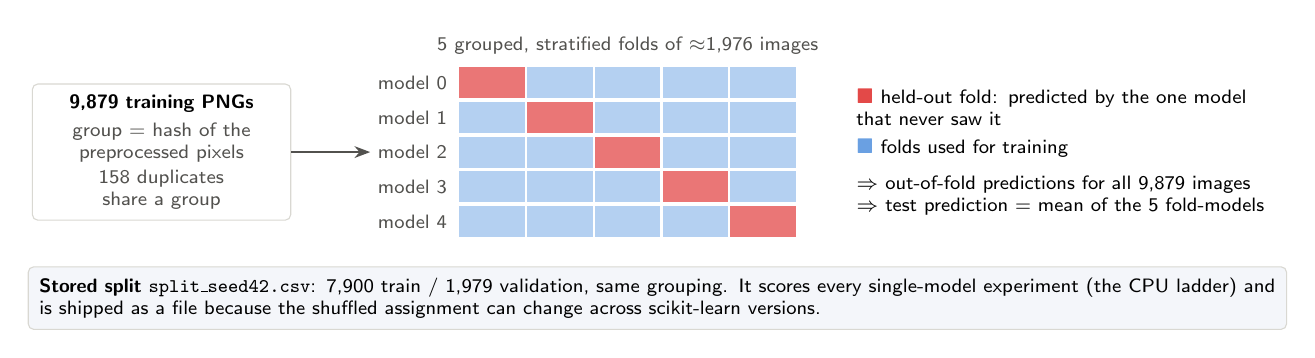
\begin{tikzpicture}[font=\sffamily\scriptsize,
    cell/.style={minimum width=8.6mm, minimum height=4.2mm, draw=white, line width=0.8pt, inner sep=0pt},
    arr/.style={-{Stealth[length=2mm]}, color=ink2, line width=0.6pt}]
    \node[draw=rule, rounded corners=2pt, align=center, inner sep=4pt, fill=white, text width=30mm] (all) at (1.7,0) {\textbf{9{,}879 training PNGs}\\[2pt]{\color{ink2}group = hash of the preprocessed pixels}\\[1pt]{\color{ink2}158 duplicates share a group}};
    \foreach \r in {0,...,4} {
      \foreach \c in {0,...,4} {
        \ifnum\r=\c \def\fc{alert!75}\else \def\fc{verified!35}\fi
        \node[cell, fill=\fc] at (5.9+\c*0.86, 0.88-\r*0.44) {};
      }
      \node[anchor=east, color=ink2] at (5.45, 0.88-\r*0.44) {model \r};
    }
    \node[color=ink2, anchor=south] at (7.62, 1.12) {5 grouped, stratified folds of $\approx$1{,}976 images};
    \draw[arr] (all.east) -- (4.35,0);
    \node[anchor=west, align=left, text width=52mm] at (10.4,0) {{\color{alert}$\blacksquare$} held-out fold: predicted by the one model that never saw it\\[2pt]{\color{verified!70}$\blacksquare$} folds used for training\\[5pt]$\Rightarrow$ out-of-fold predictions for all 9{,}879 images\\$\Rightarrow$ test prediction = mean of the 5 fold-models};
    \node[draw=rule, rounded corners=2pt, align=left, inner sep=4pt, anchor=north west, fill=panel, text width=157mm] at (0.0,-1.45) {\textbf{Stored split} \texttt{split\_seed42.csv}: 7{,}900 train / 1{,}979 validation, same grouping. It scores every single-model experiment (the CPU ladder) and is shipped as a file because the shuffled assignment can change across scikit-learn versions.};
  \end{tikzpicture}
  \caption{\textbf{Validation protocol.} Duplicates are grouped by pixel hash so that no image has a copy on the other side of a split. The final model is evaluated out-of-fold on all training images; its restriction to the stored validation split makes it directly comparable with the CPU models.}
  \label{fig:protocol}
\end{figure}

Two protocols are used. A stored split of \num{7900} training and \num{1979} validation images scores every single-model experiment. The final model is trained in five folds and reported out-of-fold on all \num{9879} images, and also on the subset that belongs to the stored validation set. Nothing was ever selected by looking at the test set. Two optional post-processing rules exist in the codebase (give a test file that is byte-identical to a training file that file's label; make identical test images share one prediction); both are off, and on the final predictions they would change 0 of \num{9879} labels, because the model already gets those images right.

% ================================================================== 3 ARCHITECTURE
\section{Architecture}
\label{sec:arch}

\subsection{Reference model trained from scratch: EmojiCNNv2}
The team's first model (30 September) had three Conv--ReLU--MaxPool blocks without normalisation and was trained with Adam at a constant learning rate of $10^{-3}$ for 20 epochs. Re-scored with its saved weights on the stored split it reaches \pct{76.71} (\num{1518} of \num{1979})\ver, with a training accuracy of only \pct{75}: it was underfitting. EmojiCNNv2 keeps the philosophy (small, from scratch, fully explainable) and fixes what held it back: BatchNorm after every convolution, a fourth stage so that the receptive field covers the 96\,px canvas, AdamW \cite{loshchilov2019adamw} with a OneCycle schedule \cite{smith2019superconvergence}, and the augmentation above (\cref{tab:v2,fig:v2arch}). It has \num{390695} parameters, costs about 0.14\,GFLOPs per image and trains at 143\,s per epoch on two CPU cores.

\begin{table}[t]
\centering\small
\caption{\textbf{EmojiCNNv2}, the reference CNN trained from scratch on $96\times96$ inputs.}
\label{tab:v2}
\begin{tabular}{@{}llrr@{}}
\toprule
Stage & Layers & Output ($C\times H\times W$) & Parameters\\
\midrule
input & RGB, normalised to $[-1,1]$ & $3\times96\times96$ & 0\\
1 & Conv $3{\times}3$ ($3\to32$) + BN + ReLU, MaxPool 2 & $32\times48\times48$ & 928\\
2 & Conv $3{\times}3$ ($32\to64$) + BN + ReLU, MaxPool 2 & $64\times24\times24$ & \num{18560}\\
3 & Conv $3{\times}3$ ($64\to128$) + BN + ReLU, MaxPool 2 & $128\times12\times12$ & \num{73984}\\
4 & Conv $3{\times}3$ ($128\to256$) + BN + ReLU & $256\times12\times12$ & \num{295424}\\
head & global average pooling, dropout 0.3, linear $256\to7$ & 7 & \num{1799}\\
\midrule
total & & & \num{390695}\\
\bottomrule
\end{tabular}
\end{table}

\begin{figure}[t]
\centering
\begin{tikzpicture}[font=\sffamily\scriptsize, x=1mm, y=1mm,
  arr/.style={-{Stealth[length=1.6mm]}, color=ink2, line width=0.55pt}]
  % helper: a feature map drawn as a slab of height h (spatial) and width w (channels)
  \newcommand{\slab}[6]{% x, h, w, colour, label top, label bottom
    \fill[#4!20, draw=#4] (#1, -#2/2) rectangle ++(#3, #2);
    \fill[#4!35, draw=#4] (#1, #2/2) -- ++(1.6,1.6) -- ++(#3,0) -- ++(-1.6,-1.6) -- cycle;
    \fill[#4!45, draw=#4] (#1+#3, -#2/2) -- ++(1.6,1.6) -- ++(0,#2) -- ++(-1.6,-1.6) -- cycle;
    \node[anchor=south, align=center] at (#1+#3/2+0.8, #2/2+2) {#5};
    \node[anchor=north, align=center, color=ink2] at (#1+#3/2, -#2/2-1) {#6};}
  \node[inner sep=0, anchor=west] (im) at (0,0) {
\includegraphics[width=16mm]{figs/vit_input.png}};
  \node[anchor=north, color=ink2] at (8,-9.5) {$3{\times}96^2$};
  \slab{22}{26}{2.2}{verified}{conv 32}{$32{\times}48^2$}
  \slab{36}{17}{3.6}{verified}{conv 64}{$64{\times}24^2$}
  \slab{51}{11}{5.4}{verified}{conv 128}{$128{\times}12^2$}
  \slab{67}{11}{8.5}{accent}{conv 256}{$256{\times}12^2$}
  \fill[alert!25, draw=alert] (86,-6) rectangle ++(2.4,12); \node[anchor=south] at (87.2,7.5) {GAP};
  \node[anchor=north, color=ink2] at (87.2,-7) {256};
  \fill[alert!45, draw=alert] (95,-3.5) rectangle ++(2.4,7); \node[anchor=south] at (96.2,5) {linear};
  \node[anchor=north, color=ink2] at (96.2,-4.5) {7};
  \foreach \a/\b in {17/21.5,26/35.5,41/50.5,58/66.5,78/85.5,90/94.5} \draw[arr] (\a,0) -- (\b,0);
  \node[align=left, anchor=west, color=ink2, text width=40mm] at (101,0) {each conv: $3{\times}3$, BatchNorm, ReLU;\\stages 1--3 end with $2{\times}2$ max-pool;\\dropout 0.3 before the linear layer;\\0.39\,M parameters in total};
\end{tikzpicture}
\caption{\textbf{EmojiCNNv2.} Spatial size halves and channel count doubles at each stage; global average pooling (GAP) turns the last $256{\times}12{\times}12$ feature map into one vector, and a linear layer gives the seven logits.}
\label{fig:v2arch}
\end{figure}


\subsection{Final model: ConvNeXt-Tiny, fine-tuned end to end}
ConvNeXt \cite{liu2022convnext} is a purely convolutional network built with the macro-design of vision transformers (\cref{fig:arch}). A $4\times4$ convolution with stride 4 turns the $224\times224$ input into a $56\times56$ grid of 96-channel patches; four stages with 3, 3, 9 and 3 blocks and widths 96, 192, 384 and 768 follow, separated by downsampling layers (LayerNorm and a $2\times2$ convolution with stride 2). A block computes
\begin{equation}
  \bm{x} \;\leftarrow\; \bm{x} + \operatorname{DropPath}\!\Big(\gamma\odot W_2\,\operatorname{GELU}\big(W_1\,\operatorname{LN}(\operatorname{DWConv}_{7\times7}(\bm{x}))\big)\Big),
\end{equation}
with $W_1$ expanding to four times the width, $W_2$ projecting back, a learned layer scale $\gamma$ and stochastic depth \cite{huang2016stochasticdepth}. Global average pooling, a LayerNorm and a linear layer produce the seven logits; the 1{,}000-way ImageNet head is discarded. With our head the network has \num{27825511} parameters, all updated during fine-tuning from the ImageNet-1k weights distributed by \texttt{timm} \cite{wightman2019timm}.

\begin{figure}[t]
  \centering
  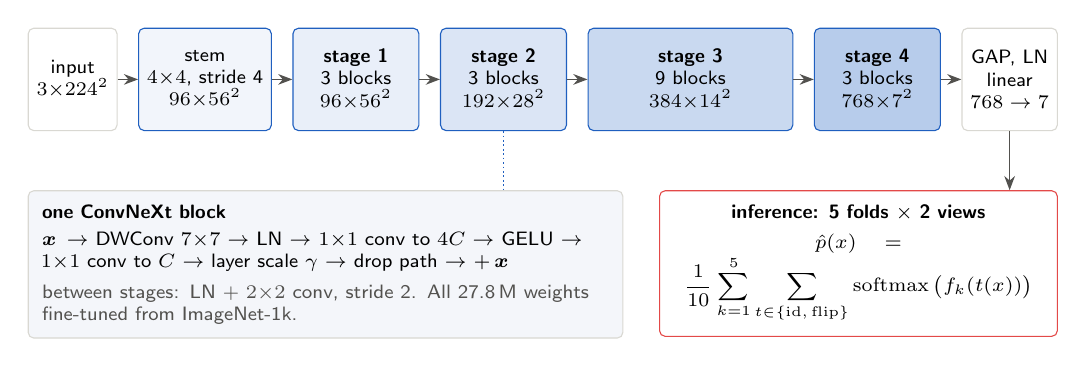
\begin{tikzpicture}[font=\sffamily\scriptsize, node distance=2.6mm,
    st/.style={draw=accent, rounded corners=2pt, align=center, minimum height=13mm, inner sep=3pt, fill=accent!#1},
    io/.style={draw=rule, rounded corners=2pt, align=center, minimum height=13mm, inner sep=3pt, fill=white},
    arr/.style={-{Stealth[length=1.8mm]}, color=ink2, line width=0.6pt}]
    \node[io] (in) {input\\$3{\times}224^2$};
    \node[st=6, right=of in] (stem) {stem\\$4{\times}4$, stride 4\\$96{\times}56^2$};
    \node[st=10, right=of stem, minimum width=16mm] (s1) {\textbf{stage 1}\\3 blocks\\$96{\times}56^2$};
    \node[st=16, right=of s1, minimum width=16mm] (s2) {\textbf{stage 2}\\3 blocks\\$192{\times}28^2$};
    \node[st=24, right=of s2, minimum width=26mm] (s3) {\textbf{stage 3}\\9 blocks\\$384{\times}14^2$};
    \node[st=32, right=of s3, minimum width=16mm] (s4) {\textbf{stage 4}\\3 blocks\\$768{\times}7^2$};
    \node[io, right=of s4] (head) {GAP, LN\\linear\\$768\to7$};
    \foreach \a/\b in {in/stem,stem/s1,s1/s2,s2/s3,s3/s4,s4/head} \draw[arr] (\a) -- (\b);
    \node[draw=rule, rounded corners=2pt, fill=panel, anchor=north west, inner sep=5pt, align=left, text width=72mm] (blk) at ($(in.south west)+(0,-0.75)$) {%
      \textbf{one ConvNeXt block}\\[2pt]
      $\bm{x}\to$ DWConv $7{\times}7$ $\to$ LN $\to$ $1{\times}1$ conv to $4C$ $\to$ GELU $\to$ $1{\times}1$ conv to $C$ $\to$ layer scale $\gamma$ $\to$ drop path $\to$ $+\,\bm{x}$\\[3pt]
      {\color{ink2}between stages: LN + $2{\times}2$ conv, stride 2. All 27.8\,M weights fine-tuned from ImageNet-1k.}};
    \draw[densely dotted, color=accent, line width=0.6pt] (s2.south) -- (s2.south |- blk.north);
    \node[draw=alert, rounded corners=2pt, align=center, inner sep=5pt, anchor=north east, text width=47mm] (ens) at ($(head.south east)+(0,-0.75)$) {\textbf{inference: 5 folds $\times$ 2 views}\\[3pt]$\displaystyle\hat p(x)=\frac{1}{10}\sum_{k=1}^{5}\sum_{t\in\{\mathrm{id},\,\mathrm{flip}\}}\operatorname{softmax}\big(f_k(t(x))\big)$};
    \draw[arr] (head.south) -- (head.south |- ens.north);
  \end{tikzpicture}
  \caption{\textbf{The final network.} ConvNeXt-Tiny with a seven-way head. One copy is trained per fold; at test time the five fold-models each see the image and its horizontal mirror and the ten softmax vectors are averaged.}
  \label{fig:arch}
\end{figure}

The team's experiment series explains the choice of this architecture at this resolution. Generic ImageNet features are not enough when frozen and read by a linear head (ResNet18 \cite{he2016resnet} as a fixed extractor: \pct{77.48}\rep). They are not useless, though: Lina concatenated frozen ResNet18 features with hand-crafted colour, transparency, edge and texture descriptors, standardised them and trained an RBF-kernel SVM ($C=10$, $\gamma$ set to \texttt{scale}), reaching \pct{96.76} on an 80/20 split (\pct{97.42} on a second split) and 0.96983 on the private leaderboard\rep, the best result obtained without fine-tuning any network. Alone, the hand-crafted descriptors reach \pct{96.05} and the frozen ResNet18 channel statistics \pct{91.65} with the same SVM\rep, so most of the gain comes from the hand-crafted style features. The hand-crafted descriptors and the non-linear classifier supply what the frozen object features miss. Fine-tuning the whole backbone adapts the filters to rendering style (the same ResNet18 fine-tuned: \pct{93.72}\rep). ConvNeXt-Tiny beat ResNet18 and EfficientNet-B0 \cite{tan2019efficientnet} at the same 128\,px input (\pct{95.90} against \pct{93.72} and \pct{93.12}\rep), which we attribute to its large depthwise kernels and LayerNorm capturing stroke and shading over a wider context. Input resolution then gave the largest single gain (\pct{97.57} at 224\,px\rep): 224\,px is the pre-training resolution and is close to the 240\,px native size of the Facebook, Messenger and Mozilla files, which are therefore barely resampled.

\subsection{Training recipe, ensemble and test-time augmentation}
\Cref{tab:recipe} gives both recipes. The final model is trained with AdamW (learning rate $2\times10^{-4}$, weight decay 0.05) under a OneCycle schedule over 10 epochs with batches of 32, stochastic depth 0.1, plain cross-entropy and mixed precision \cite{micikevicius2018mixed}. Seeds are 42 plus the fold index with deterministic cuDNN kernels. One model is trained per fold and validated on the fold it never saw; the weights kept are those of the last epoch (\cref{sec:epoch} shows why). Predictions are averaged in probability space (soft voting) \cite{lakshminarayanan2017ensembles}, so that one confident fold cannot be outvoted by three unsure ones.

\begin{table}[t]
\centering\small
\caption{\textbf{Training recipes} of the reference CNN and of the final model.}
\label{tab:recipe}
\begin{tabularx}{\textwidth}{@{}l>{\raggedright\arraybackslash}X>{\raggedright\arraybackslash}X@{}}
\toprule
 & EmojiCNNv2 (reference) & ConvNeXt-Tiny (final)\\
\midrule
Input & $96\times96$, $[-1,1]$ & $224\times224$, ImageNet mean and std\\
Initialisation & random & ImageNet-1k (\texttt{convnext\_tiny.fb\_in1k})\\
Optimiser & AdamW, lr $2\times10^{-3}$, weight decay $10^{-4}$ & AdamW, lr $2\times10^{-4}$, weight decay 0.05\\
Schedule & OneCycle, 25 epochs, batch 64 & OneCycle, 10 epochs per fold, batch 32\\
Regularisation & BatchNorm, dropout 0.3, flip + shift & stochastic depth 0.1, flip + shift\\
Loss & cross-entropy & cross-entropy, no label smoothing\\
Checkpoint kept & lowest validation loss & last epoch (run B, final); lowest validation loss (run A, ablation)\\
Validation & stored split (\num{7900} / \num{1979}) & 5-fold grouped CV, out-of-fold on \num{9879}\\
Inference & single pass & mean of 5 models $\times$ \{image, mirror\}\\
Hardware & 2 CPU cores, fp32 & NVIDIA RTX 4090 (RunPod), mixed precision\\
\bottomrule
\end{tabularx}
\end{table}

\subsection{A self-supervised transformer: DINOv2}
\label{sec:dino}
Besides convolutional networks, the team tried a vision transformer \cite{dosovitskiy2021vit}. DINOv2 \cite{oquab2024dinov2} is a ViT pretrained without labels on LVD-142M, a curated set of about 142 million images, by self-distillation: a student network learns to reproduce a teacher's output on different crops of the same image. With a patch size of 14, a $224\times224$ input becomes a $16\times16$ grid of tokens processed by global self-attention. Its features are among the strongest general-purpose ones available, which made it the natural candidate for a model that needs no task-specific design. The plan was to use the newer DINOv3; its official weights required an access approval that did not arrive in time, so the run used DINOv2.

\paragraph{Setup} Lina ran this branch; the code, configurations and results are in \nolinkurl{members/lina-oumhand/dinov2-partial-finetune/} of the repository\rep. The model was DINOv2 ViT-S/14 (22\,M parameters). Its first ten transformer blocks were frozen and their tokens cached; the last two blocks, the final LayerNorm and a linear head were trained. The head read the class token concatenated with the mean patch token (768 values). Images were composited on white and letterboxed to 224\,px with Lanczos resampling, without augmentation. The split held 7{,}903 images for training and 1{,}976 for development, with exact duplicates grouped. AdamW used a learning rate of $3\times10^{-5}$ for the backbone and $10^{-3}$ for the head, weight decay 0.01 and batch 16 under a cosine schedule. Training stopped after seven epochs, and epoch 3 was kept.

\paragraph{Results} The model scored \pct{95.90} on the development images (1{,}895 of 1{,}976; macro F1 0.959) and 0.95607 on the private leaderboard. Averaging the image and its mirror added one image (\pct{95.95}). A ConvNeXt-Tiny tuned the same way, with only its last stage trainable, reached \pct{95.55}. The equal average of the two reached \pct{97.12} on the development images but 0.96477 on the private leaderboard, 0.6 points lower. The development images had been reused for earlier choices in this branch, so its estimates were optimistic, the opposite of our grouped out-of-fold protocol, whose private score came out \emph{above} the estimate (\cref{sec:kaggle}).

\paragraph{Why it trailed ConvNeXt} The simplest explanation is budget: only 2 of 12 blocks were trained, while our ConvNeXt was fine-tuned end to end, and \cref{sec:journey} shows how much full fine-tuning matters here. Two further reasons are plausible but untested. First, the DINO objective that DINOv2 builds on trains features to be invariant to colour jittering, Gaussian blur and solarization \cite{caron2021dino}: precisely the palette, gradient and anti-aliasing cues that separate vendors. Second, geometry: a 72\,px emoji upscaled to 224\,px puts about 4.5 native pixels in each 14\,px patch, and the first layer of a ViT mixes outline, fill and edge pixels into one token, whereas ConvNeXt's $4\times4$ stem covers about 1.3 native pixels and its $7\times7$ depthwise kernels keep strokes separate in the early layers.

\subsection{Combining backbones: from voting to learned fusion}
\label{sec:fusion}
Our final model combines members of the same architecture by soft voting (\cref{fig:arch}). The team also explored combining \emph{different} backbones, on the logic of \cref{sec:background}: an ensemble helps only if its members make different mistakes, and a self-supervised transformer and a supervised CNN see an image very differently. \Cref{fig:fusion} shows the two ways to combine them. In late fusion (soft voting) each backbone produces its own class probabilities and these are averaged. In learned fusion, each frozen backbone produces a feature vector, a linear layer projects it to a common width so that it becomes one token, and a small trainable transformer attends across the tokens, in effect translating each backbone's representation into a shared space before a class token makes the decision. Only the projection layers and the fusion transformer are trained, which keeps the number of trainable parameters small, and as with stacking the fusion model must be trained on data the backbones were not fine-tuned on.

\begin{figure}[t]
\centering
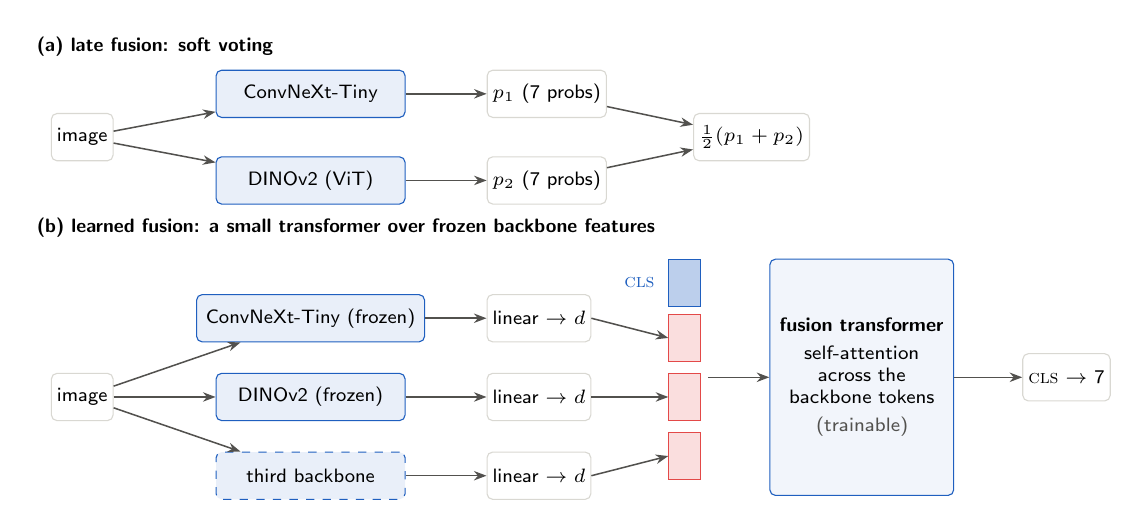
\begin{tikzpicture}[font=\sffamily\scriptsize, node distance=3mm,
  bb/.style={draw=accent, rounded corners=2pt, fill=accent!10, minimum width=24mm, minimum height=6mm, align=center},
  fz/.style={draw=rule, rounded corners=2pt, fill=white, minimum height=6mm, align=center, inner sep=2pt},
  tk/.style={draw=alert, fill=alert!18, minimum width=4mm, minimum height=6mm, inner sep=0},
  arr/.style={-{Stealth[length=1.6mm]}, color=ink2, line width=0.55pt}]
  \node[font=\sffamily\scriptsize\bfseries, anchor=west] at (0,1.15) {(a) late fusion: soft voting};
  \node[fz] (x1) at (0.7,0) {image};
  \node[bb] (b1) at (3.6,0.55) {ConvNeXt-Tiny};
  \node[bb] (b2) at (3.6,-0.55) {DINOv2 (ViT)};
  \node[fz] (p1) at (6.6,0.55) {$p_1$ (7 probs)};
  \node[fz] (p2) at (6.6,-0.55) {$p_2$ (7 probs)};
  \node[fz] (avg) at (9.2,0) {$\tfrac12(p_1+p_2)$};
  \foreach \u/\v in {x1/b1,x1/b2,b1/p1,b2/p2,p1/avg,p2/avg} \draw[arr] (\u) -- (\v);
  \begin{scope}[yshift=-3.3cm]
  \node[font=\sffamily\scriptsize\bfseries, anchor=west] at (0,2.15) {(b) learned fusion: a small transformer over frozen backbone features};
  \node[fz] (y) at (0.7,0) {image};
  \node[bb] (c1) at (3.6,1.0) {ConvNeXt-Tiny (frozen)};
  \node[bb] (c2) at (3.6,0) {DINOv2 (frozen)};
  \node[bb, dashed] (c3) at (3.6,-1.0) {third backbone};
  \foreach \k/\n in {1/1.0,2/0,3/-1.0} { \node[fz] (pr\k) at (6.5,\n) {linear $\to d$}; \draw[arr] (y) -- (c\k); \draw[arr] (c\k) -- (pr\k); }
  \node[tk, draw=accent, fill=accent!30] (cls) at (8.35,1.45) {};
  \node[left=0.5mm of cls, color=accent] {\textsc{cls}};
  \foreach \k/\n in {1/0.75,2/0,3/-0.75} { \node[tk] (t\k) at (8.35,\n) {}; \draw[arr] (pr\k.east) -- (t\k.west); }
  \node[draw=accent, rounded corners=2pt, fill=accent!6, minimum height=30mm, text width=21mm, align=center] (tf) at (10.6,0.25) {\textbf{fusion transformer}\\[2pt]self-attention across the backbone tokens\\[2pt]{\color{ink2}(trainable)}};
  \draw[arr] (8.65,0.25) -- (tf.west);
  \node[fz] (out) at (13.2,0.25) {\textsc{cls} $\to$ 7};
  \draw[arr] (tf) -- (out);
  \end{scope}
\end{tikzpicture}
\caption{\textbf{Two ways to combine different backbones.} (a) Averaging the class probabilities, which is what our final ConvNeXt ensemble does across folds. (b) Learned fusion: each backbone's feature vector becomes one token, and a small trainable transformer learns how to weigh and combine them. The dashed box is the third member of the team's experiment (see the note below).}
\label{fig:fusion}
\end{figure}

The only recorded result of this line of work is the DINOv2 + ConvNeXt entry in \cref{tab:kaggle}: 0.96477 on the private leaderboard, against 0.98218 for ConvNeXt-Tiny alone. Whatever the combiner, adding a member that is clearly weaker on this task pulled the stronger model down, which is the outcome the ensemble literature predicts when one member's errors dominate.

\begin{tcolorbox}[enhanced,colback=alert!6,colframe=alert!60,arc=2pt,boxrule=0.6pt,left=6pt,right=6pt,top=4pt,bottom=4pt,fonttitle=\sffamily\bfseries\small,title={To complete before submission (Adam)}]
\small The configuration of the three-backbone fusion experiment was run outside the submitted codebase and is not recorded in our files: which third backbone was used, whether the transformer fused features or probabilities, its size and training data, and whether the 0.96477 entry came from the fusion model or from a vote. Fill these in from the Codex session (see \texttt{members/adam-zeraiki/README.md} in the repository), or delete this box and the dashed member of \cref{fig:fusion}(b).
\end{tcolorbox}


% ================================================================== 4 METRICS
\section{Metrics chosen}
\label{sec:metrics}
Accuracy is the competition metric and our headline number, but alone it hides two things we care about. We therefore report:
\begin{itemize}[leftmargin=1.2em]
  \item \textbf{Accuracy with its uncertainty.} With $n$ images the binomial standard error is $\sqrt{a(1-a)/n}$: about 0.65 points at \pct{91} and 0.4 points at \pct{97} on the \num{1979}-image split, 0.15 points out-of-fold on \num{9879} images. We add 95\% bootstrap intervals (\num{2000} resamples) for the final model.
  \item \textbf{Macro F1 and balanced accuracy} (mean per-class recall). Messenger and Mozilla together are \pct{9.9} of the data; these metrics make a drop on a small class visible.
  \item \textbf{Per-class recall and the confusion matrix}, because the errors have structure (export families, look-alike vendors).
  \item \textbf{Log loss} $-\frac1n\sum_i\log\hat p_{i,y_i}$ and the \textbf{expected calibration error} $\mathrm{ECE}=\sum_b\frac{|B_b|}{n}\,|\mathrm{acc}(B_b)-\mathrm{conf}(B_b)|$ over 15 confidence bins \cite{guo2017calibration}, to see whether the probabilities are trustworthy.
  \item \textbf{Paired tests.} When two models are scored on the same images we report the counts of images only one of them gets right and an exact McNemar test \cite{mcnemar1947,dietterich1998tests}, because two accuracies alone do not say whether the models fail on the same images.
\end{itemize}

% ================================================================== 5 PERFORMANCE
\section{Performance}
\label{sec:perf}

\subsection{How we got to the final model}
\label{sec:journey}
The final model was not designed in one step. \Cref{tab:journey} tells the project in the order it happened: each row is something we tried, what it gave, and what that taught us, which is what decided the next row. The complete list of runs with their settings is in \cref{app:log,app:who}.

\begin{table}[p]
\centering\small
\caption{\textbf{From first try to final model.} Accuracies are validation accuracies unless marked $^\dagger$ (private leaderboard). \ver\ verified by the codebase, \rep\ from Erdem's log, the experiment records in the repository or Kaggle; $^\S$ on the DINOv2 branch's development split.}
\label{tab:journey}
\renewcommand{\arraystretch}{1.18}
\newcommand{\stp}[1]{\tikz[baseline=(n.base)]\node[circle, fill=accent, text=white, inner sep=1.2pt, minimum size=4.2mm, font=\sffamily\scriptsize\bfseries](n){#1};}
\begin{tabularx}{\textwidth}{@{}c>{\raggedright\arraybackslash}p{44mm}>{\raggedleft\arraybackslash}p{17mm}>{\raggedright\arraybackslash}X@{}}
\toprule
 & What we tried & Result & What we learned, and what we changed\\
\midrule
\stp{1} & First CNN: 3 conv blocks, no normalisation, Adam at a constant $10^{-3}$, 20 epochs (30 Sept.) & 76.71\%\ver & Training accuracy only 75\%: the model underfits. \textbf{Next:} BatchNorm, a fourth stage and a OneCycle schedule.\\
\stp{2} & EmojiCNNv2 (0.39\,M parameters), same data & 90.96\%\ver & +14 points from optimisation and normalisation alone, no extra data. A good CNN from scratch is a strong baseline.\\
\stp{3} & File metadata only (size, PNG mode, hidden colour), random forest & 87.37\%\ver & The file format leaks the label. \textbf{Next:} composite on white, square canvas, exact-pixel augmentation; keep the final model pixel-only. Same CNN with compositing: 92.11\% $\to$ 93.62\%\rep.\\
\stp{4} & Hand-crafted features: colour histogram + HOG with an SVM (Erdem); extra-trees on pixels, colour and transparency (Lina) & 81.28\%, 82.14\%\rep & Below every trained CNN: the cues are too fine for generic descriptors. \textbf{Next:} learn the features.\\
\stp{5} & Pretrained ResNet18 as a frozen feature extractor: linear head (Erdem); with hand-crafted style features and an RBF SVM (Lina) & 77.48\%, 96.76\%\rep & ImageNet features describe objects, not drawing style; frozen, they need hand-crafted style descriptors to compete. \textbf{Next:} fine-tune the whole network.\\
\stp{6} & Full fine-tuning at 128\,px: ResNet18, EfficientNet-B0, ConvNeXt-Tiny; ResNet18 at 160\,px with file-format features (Charles) & 93.72\%, 93.12\%, 95.90\%\rep; 0.96396$^\dagger$ & Fine-tuning recovers 16 points; ConvNeXt is best. Charles's entry also reads the file format, so it is not a pixels-only result. \textbf{Next:} build on ConvNeXt-Tiny.\\
\stp{7} & Stronger augmentation: rotation, scaling, label smoothing & 94.38\%\rep & $-1.5$ points: resampling blurs the outlines that identify a vendor. \textbf{Next:} flips and integer shifts only.\\
\stp{8} & Input resolution 128 $\to$ 224\,px & 97.57\%\rep & +1.7 points, the largest single gain: resolution matters more than architecture.\\
\stp{9} & Ensembles (128 + 224\,px), retraining on all data, nearest-neighbour upscaling (E15, Erdem) & 97.93\%\rep; 0.98238$^\dagger$ & Retraining on all data changed the private score by +0.14 and $-0.08$ points: no reliable gain. The best entry mixes resolutions and resize filters; in a controlled test at 144\,px, nearest-neighbour instead of bicubic resizing gave +0.9 points (E12a, E12b\rep); at 216\,px nearest-neighbour did no better than 224\,px bicubic (E13, E8\rep).\\
\stp{10} & Self-supervised ViT: DINOv2 ViT-S/14, last 2 of 12 blocks tuned (Lina); averaged with a partially tuned ConvNeXt & 95.90\%, 97.12\%$^\S$; 0.95607$^\dagger$, 0.96477$^\dagger$ & The transformer is weaker here, and the average fell 0.6 points from its development estimate to the leaderboard (reused development split). \textbf{Next:} try learning the combination.\\
\stp{11} & Learned fusion of DINOv2, ConvNeXt and 1{,}460 style features (transformer and MLP heads); decision models Julia-1 and Jev & best 97.01\%$^\S$ vs 97.12\% & No combiner beat the plain average; Jev fixed 8 errors and made 37. \textbf{Next:} back to one strong architecture, fine-tuned end to end.\\
\stp{12} & ConvNeXt-Tiny, 5 grouped folds, flip TTA, lowest-validation-loss epoch (run A) & 97.29\%\ver & Validation loss and accuracy disagree. \textbf{Next:} keep the last epoch of the schedule.\\
\rowcolor{panel}\stp{13} & Same, last epoch (run B): \textbf{final model} & 97.69\%\ver; 0.98218$^\dagger$ & +0.40 points over run A ($p=2.4\times10^{-5}$), 13 minutes of training.\\
\bottomrule
\end{tabularx}
\end{table}

Three turns shaped the project. The first was finding the file-format shortcut (step 3): it changed the question from ``how high can we score'' to ``how high can we score from the drawing'', and every later comparison was made under that rule. The second was the failure of frozen features (step 5), which showed that vendor style is not what ImageNet pretraining encodes, and that the backbone has to be adapted. The third was the gap between validation loss and accuracy at the end (step 12), which changed how we choose a checkpoint. Several ideas did not work, and they are as informative as the ones that did: resampling augmentation, retraining on all data, adding a weaker transformer to a strong CNN, and learned fusion or decision models on top of two networks and hand-crafted style features all lost or failed to gain accuracy (\cref{sec:nowork,sec:fusion}); only an expert that reads the file bytes, combined by simple rules, added accuracy.

\subsection{Experiment ladder}
\label{sec:ladder}


\begin{table}[t]
\centering\small
\caption{\textbf{Validation results of every model.} Verified rows (\ver) were produced by the submitted codebase on the stored split or out-of-fold (OOF); reported rows (\rep) come from the team's log on an 80/20 split of about \num{1976} images and are only roughly comparable. $^\ast$Macro precision, the only macro metric in that log.}
\label{tab:ladder}
\setlength{\tabcolsep}{4.5pt}
\begin{tabular}{@{}llrrc@{}}
\toprule
Model & Input & Accuracy & Macro F1 & \\
\midrule
Majority class (always Apple) & none & 19.61\% & & \ver\\
File format only: size, mode, alpha flag (random forest) & no pixels & 66.40\% & & \ver\\
File metadata incl.\ hidden colour (random forest) & no drawing & 87.37\% & 0.867 & \ver\\
Colour histogram + HOG, RBF SVM (E1b) & 64\,px & 81.28\% & 0.848$^\ast$ & \rep\\
Extra-trees on pixels, colour histograms, transparency (Lina) & resized & 82.14\% & & \rep\\
\midrule
Baseline CNN, 30 September (3 blocks, no BN, Adam) & 96\,px & 76.71\% & 0.738 & \ver\\
Simple CNN, white compositing (E3) & 96\,px & 93.62\% & 0.933$^\ast$ & \rep\\
EmojiCNNv2, pixels only & 96\,px & 90.96\% & 0.907 & \ver\\
EmojiCNNv2 + 8 file-format features (late fusion, ablation) & 96\,px & 93.38\% & 0.926 & \ver\\
\midrule
ResNet18, frozen features, linear head (E4) & 128\,px & 77.48\% & & \rep\\
ResNet18 frozen + hand-crafted features, RBF SVM (Lina) & & 96.76\% & & \rep\\
ResNet18, fine-tuned (E5) & 128\,px & 93.72\% & & \rep\\
EfficientNet-B0, fine-tuned (E6) & 128\,px & 93.12\% & & \rep\\
ConvNeXt-Tiny, fine-tuned (E6b) & 128\,px & 95.90\% & & \rep\\
ConvNeXt-Tiny + rotation/scale aug.\ + label smoothing (E7) & 128\,px & 94.38\% & & \rep\\
ConvNeXt-Tiny, fine-tuned (E8) & 224\,px & 97.57\% & & \rep\\
Ensemble ConvNeXt-Tiny 128 + 224\,px (E9) & both & 97.93\% & & \rep\\
\midrule
ConvNeXt-Tiny, 5 folds, TTA, lowest-val-loss epoch (run A, ablation) & 224\,px & 97.29\% OOF & 0.972 & \ver\\
\rowcolor{panel}\textbf{ConvNeXt-Tiny, 5 folds, TTA, last epoch (run B): final model} & 224\,px & \textbf{97.69\%} OOF & \textbf{0.977} & \ver\\
\quad same model, restricted to the stored \num{1979}-image split & & 97.07\% & 0.969 & \ver\\
Both checkpoints of every fold averaged (10 checkpoints, ablation) & 224\,px & 97.70\% OOF & 0.977 & \ver\\
\bottomrule
\end{tabular}
\end{table}

\Cref{tab:ladder} and \cref{fig:ladder} list every model of the project; each rung changes one thing. The file metadata alone set a high bar: \pct{87.4} without seeing the drawing, which any pixel model should clear before it can claim to have learned style. The September CNN does not (\pct{76.71}). EmojiCNNv2 reaches \pct{90.96} with BatchNorm, a fourth stage, OneCycle and exact-pixel augmentation and nothing else; on the same \num{1979} images it is right on 346 images the baseline gets wrong and wrong on only 64 that the baseline gets right (exact McNemar $p<10^{-40}$). Adding the eight file-format features by late fusion gives \pct{93.38} (79 images right only with fusion, 31 only without; $p = 5.3\times10^{-6}$). That 2.4-point gain is the price of keeping the final model pixel-only; we consider it well spent, since it is the part of the score that comes from the encoder rather than the artist. The pretrained backbones then take over, with resolution as the decisive variable.

\begin{figure}[t]
  \centering
  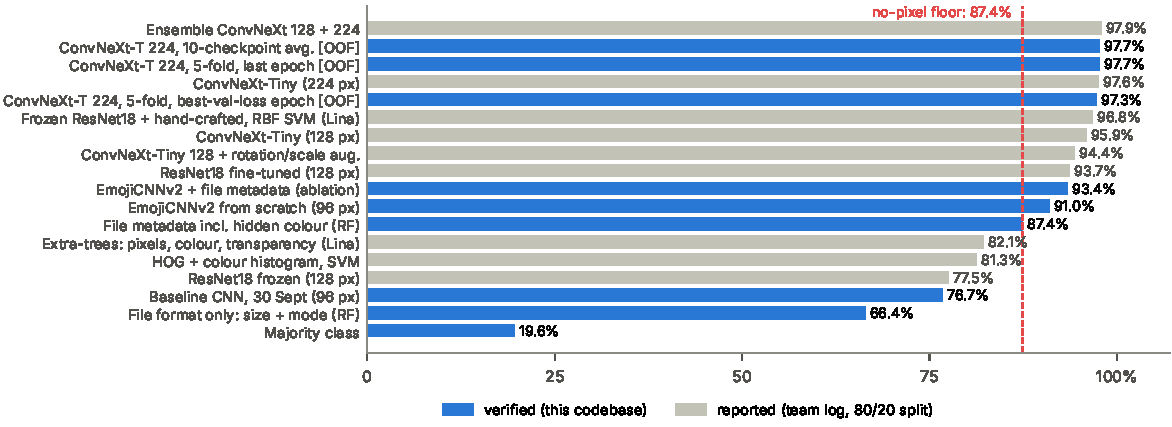
\includegraphics[width=\textwidth]{figs/fig5_ladder.pdf}
  \caption{\textbf{The experiment ladder.} Validation accuracy of every model in the project, sorted. Blue bars were produced by the submitted codebase (stored split or out-of-fold), grey bars come from the team's log on a different 80/20 split. The dashed line is the accuracy a random forest reaches from file metadata alone: the September CNN, the hand-crafted classifiers and frozen ResNet18 with a linear head sit below it; every BatchNorm or fine-tuned CNN, and frozen ResNet18 with hand-crafted features and an SVM, sit above.}
  \label{fig:ladder}
\end{figure}

\subsection{Final model}
\label{sec:final}
The final model reaches an out-of-fold accuracy of \textbf{\pct{97.69}} (\num{9651} of \num{9879} images; 95\% bootstrap CI [97.40, 97.98]), balanced accuracy 0.9762, macro F1 0.9773 and log loss 0.1105\ver. Restricted to the stored validation split it scores \pct{97.07} (\num{1921} of \num{1979}), the number to compare with the CPU rows of \cref{tab:ladder}. The five folds range from \pct{97.47} to \pct{97.87} (\cref{tab:folds}), the spread expected from folds of about \num{1976} images. Recall is above \pct{96} for every vendor (\cref{tab:perclass}); the smallest class, Messenger, is among the best recognised (\pct{98.8}).

\begin{table}[t]
\centering\small
\begin{minipage}[t]{0.56\textwidth}\vspace{0pt}
\caption{\textbf{Per-fold results} (flip TTA). Both runs share every training batch; only the epoch kept differs.}
\label{tab:folds}
\begin{tabular}{@{}crrcrc@{}}
\toprule
 & \multicolumn{2}{c}{Run A (lowest val.\ loss)} & & \multicolumn{2}{c}{Run B (last epoch)}\\
\cmidrule{2-3}\cmidrule{5-6}
Fold & Accuracy & Epoch & & Accuracy & Min.\\
\midrule
0 & 97.67\% & 7 & & 97.87\% & 2.9\\
1 & 96.76\% & 4 & & 97.47\% & 2.4\\
2 & 97.42\% & 6 & & 97.67\% & 2.7\\
3 & 96.81\% & 5 & & 97.62\% & 2.6\\
4 & 97.77\% & 8 & & 97.82\% & 2.4\\
\midrule
OOF & 97.29\% & & & \textbf{97.69\%} & 13.0\\
\bottomrule
\end{tabular}
\end{minipage}\hfill
\begin{minipage}[t]{0.4\textwidth}\vspace{0pt}
\caption{\textbf{Per-vendor metrics} of the final model, out-of-fold.}
\label{tab:perclass}
\begin{tabular}{@{}lrrr@{}}
\toprule
Vendor & Prec. & Recall & F1\\
\midrule
Apple     & 0.952 & 0.967 & 0.960\\
Facebook  & 0.991 & 0.977 & 0.984\\
Google    & 0.968 & 0.987 & 0.977\\
Messenger & 0.979 & 0.988 & 0.984\\
Mozilla   & 0.982 & 0.962 & 0.972\\
Samsung   & 0.984 & 0.990 & 0.987\\
WhatsApp  & 0.992 & 0.964 & 0.978\\
\bottomrule
\end{tabular}
\end{minipage}
\end{table}

\subsection{Which epoch to keep}
\label{sec:epoch}
Our first five-fold run (run A) followed the usual rule and kept, for each fold, the epoch with the lowest validation loss. It chose epochs 7, 4, 6, 5 and 8, while validation accuracy was still rising at epoch 10 (\cref{fig:dynamics}). Run B kept the last epoch of the OneCycle schedule, where the learning rate has been annealed to zero; this rule involves no selection on the validation set at all. Run B re-trained the five folds from the same seeds on the same GPU, and the two runs reproduced each other to the last decimal at every epoch, so the difference between them is entirely the epoch that was kept. Run B is better by 0.40 points out-of-fold (\pct{97.69} against \pct{97.29}; 95\% paired bootstrap CI [0.22, 0.59]); on the same \num{9879} images 64 are right only under run B and 24 only under run A (exact McNemar $p = 2.4\times10^{-5}$).

\begin{figure}[t]
  \centering
  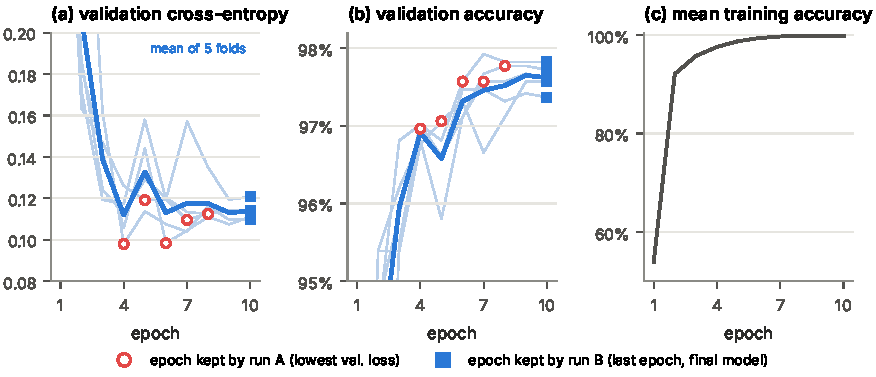
\includegraphics[width=\textwidth]{figs/fig7_dynamics.pdf}
  \caption{\textbf{Validation loss and accuracy disagree on when to stop.} Thin lines are the five folds, the thick line their mean. (a) Validation cross-entropy is lowest around epochs 4 to 8, where run A stopped (circles). (b) Validation accuracy keeps improving until the end of the schedule, where run B stopped (squares). (c) Training accuracy saturates at \pct{99.9} by epoch 8: the network is still sharpening its decisions, not learning new ones.}
  \label{fig:dynamics}
\end{figure}

The reason is over-confidence \cite{guo2017calibration}. Once almost every image is right, the cross-entropy is dominated by a handful of confident mistakes: in the final model \pct{96} of the total log loss comes from the \pct{2.3} of images it gets wrong. Later epochs push every probability towards one; this fixes borderline images (accuracy rises) and makes the remaining mistakes more confident (loss rises). \Cref{fig:calibration} shows both effects. Run B's mean confidence on its errors is 0.86 against 0.77 for run A, and 71 of its errors are made with more than \pct{99} confidence against 40; its calibration error is slightly higher (ECE \pct{1.61} against \pct{1.24}), yet it is more accurate at every coverage level. For a metric that only counts correct labels, the last epoch is the right choice. We also averaged both snapshots of every fold, ten checkpoints in all, in the spirit of weight or snapshot averaging \cite{izmailov2018swa}: \pct{97.70} out-of-fold, a tie with run B, and slightly lower on both leaderboards (\cref{sec:kaggle}). Giving half the vote to less-converged weights does not help, so the final model is the five last-epoch fold-models: the simpler rule and the better number.

\begin{figure}[t]
  \centering
  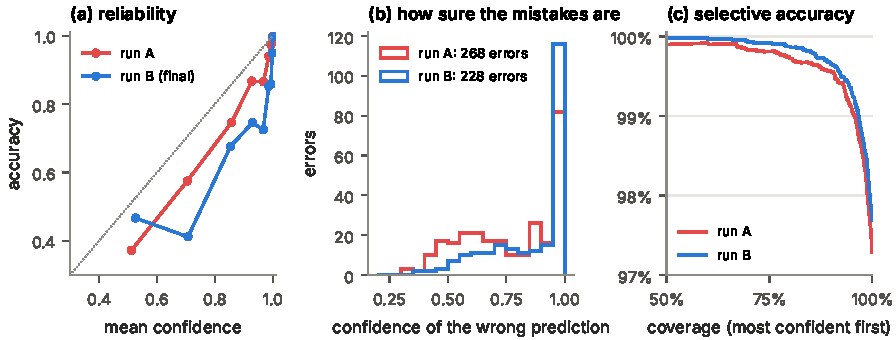
\includegraphics[width=\textwidth]{figs/fig8_calibration.pdf}
  \caption{\textbf{More accurate and more over-confident.} Out-of-fold predictions of run A (lowest-validation-loss epoch) and run B (last epoch, final model). (a) Reliability diagram: both runs are over-confident below \pct{99} confidence. (b) Confidence of the wrong predictions: run B makes fewer mistakes, and more of them with near-certain probability, which is what raises its log loss. (c) Accuracy of the most confident fraction of images: run B is above run A at every coverage; at confidence $\ge 0.99$ it still covers \pct{95.3} of the images at \pct{99.25} accuracy.}
  \label{fig:calibration}
\end{figure}

\subsection{Is there a double descent?}
\label{sec:descent}
Classical learning theory predicts a U-shaped test error: it falls while a model fits the signal and rises once it starts to fit noise. Belkin et al.\ showed that beyond the interpolation threshold, the capacity at which a model fits its training set exactly, test error can fall a second time, a shape they called double descent \cite{belkin2019doubledescent}. Nakkiran et al.\ found it in deep networks both as a function of model size and of training time: in \emph{epoch-wise} double descent, test error peaks when a model has been trained just long enough to reach near-zero training error and falls again if training continues, most strongly when training labels are noisy \cite{nakkiran2020deepdd}.

Our curves contain two non-monotonic shapes (\cref{fig:descent}). The clearest is in EmojiCNNv2 (panels a and b). Validation loss falls for three epochs, climbs from 1.16 to 2.15 by epoch 7 while validation accuracy drops from \pct{55} at epoch 2 to \pct{43}, then descends a second time to 0.31; training loss decreases at every epoch. It looks like a double descent, but it is not the one described above. At the peak the network fits only \pct{74} of its training images, far from interpolation, and the rise coincides with the warm-up of the OneCycle schedule, whose learning rate reaches its maximum at epochs 6 and 7 (panel c). The validation curve keeps oscillating while the learning rate stays high and settles as it anneals; the fusion model, trained with the same schedule, oscillates over the same epochs. We therefore read it as optimisation instability at a large learning rate, not as a capacity effect. A likely contributor, which we did not isolate, is BatchNorm \cite{ioffe2015batchnorm}: validation uses running statistics that lag behind weights that are changing quickly, so the validation pass sees a slightly different network from the one the training loss measures.

\begin{figure}[t]
  \centering
  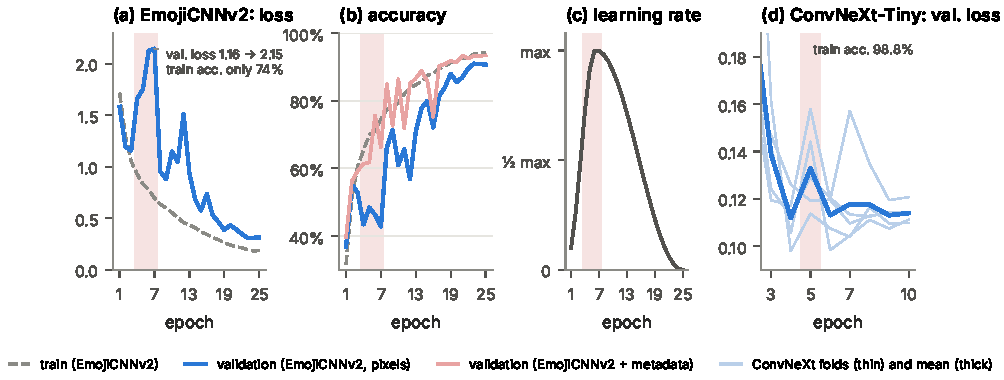
\includegraphics[width=\textwidth]{figs/fig15_second_descent.pdf}
  \caption{\textbf{A second descent that is not (clearly) double descent.} (a, b) EmojiCNNv2 on the stored split: validation loss rises and accuracy falls between epochs 3 and 7 (shaded) while training loss keeps decreasing and training accuracy is only \pct{74}. (c) The rise coincides with the peak of the OneCycle learning rate. (d) ConvNeXt-Tiny, run A: a small bump at epoch 5, when training accuracy is already \pct{98.8}, in the regime where epoch-wise double descent is reported \cite{nakkiran2020deepdd}, but too small to separate from noise.}
  \label{fig:descent}
\end{figure}

ConvNeXt-Tiny shows a much smaller bump (panel d): the mean validation loss rises from 0.112 at epoch 4 to 0.133 at epoch 5 and returns to 0.113 at epoch 6, and validation accuracy dips in four of the five folds (from \pct{96.91} to \pct{96.58} on average). Here training accuracy is already \pct{98.8}, close to the regime where epoch-wise double descent appears. The shape is consistent with it, but a 0.3-point dip from a single seed is within the epoch-to-epoch noise of a 1{,}976-image fold (standard error about 0.4 points), so we do not claim it. Model-wise double descent would need a sweep of width or depth under a fixed recipe; our ladder changes several factors at once and cannot be read that way. The practical lesson holds for both networks: stopping at the first minimum of the validation loss would have kept EmojiCNNv2 at \pct{53} accuracy (epoch 3) instead of \pct{91}, which is why the codebase never stops early under OneCycle, and it echoes the conclusion of \cref{sec:epoch} reached from the calibration side.

\paragraph{A controlled test: 2{,}000 and 4{,}000 epochs} Adam had read the deep double descent paper of Nakkiran et al.\ \cite{nakkiran2020deepdd} out of curiosity, and we wanted to know whether its findings apply to a task like ours. To test for double descent directly, on 28 October we repeated its protocol on our data. A pre-activation ResNet18 whose four stages have $k$, $2k$, $4k$ and $8k$ channels ($k=64$ is the standard network, \num{11170631} parameters) was trained from scratch on $32\times32$ images, alpha composited on white, with Adam at a constant learning rate of $10^{-4}$, batch 128, random crops and flips, for 2{,}000 epochs with no schedule and no early stopping, on the DINOv2 branch's 7{,}903 / 1{,}976 grouped split. A fixed random 10\% or 20\% of the training labels was replaced by a wrong class; development labels stay clean. A first batch (width 64 at 0, 10 and 20\% noise; widths 4, 8, 16 and 32 at 20\%) took 70 minutes on one RTX 4090; a second batch added widths 3, 5, 6, 7, 10 and 12, widths 6 and 8 on half of the training images, and width 64 at 20\% noise for 4{,}000 epochs (\$2.42 of GPU time in all)\rep. \Cref{fig:dd2000} shows the result. With 20\% wrong labels the width-64 network follows the epoch-wise shape: development error (smoothed over 25 epochs) falls to its minimum of \pct{35.3} at epoch 25, before the corrupted labels are learnt, rises to \pct{39.2} by epoch 214 while the network memorises 95\% of them, then descends a second time, slowly, to about \pct{37.3} by epoch 1{,}500 without returning to the first minimum. The 4{,}000-epoch run repeats the shape (minimum \pct{34.8} at epoch 26, peak \pct{39.1} at epoch 214) and shows that the second descent stops there: from epoch 1{,}500 to 4{,}000 the smoothed error stays between 36.3 and \pct{38.7}, ending at \pct{37.3}. Doubling the training time bought nothing. Widths 32 and 16 trace the same shape (second descents of 1.9 and 1.2 points). With 10\% noise the bump is barely visible, and with clean labels there is none: error keeps falling long after the training set is fitted, from \pct{22.4} at epoch 100, when training accuracy reaches 99\%, to \pct{20.1} at epoch 2{,}000. Across 11 widths at 20\% noise the error at the end of training falls steadily, from \pct{48.4} at $k=3$ to \pct{37.5} at $k=64$, while the share of training labels the network fits rises from 67\% to 99\%; the interpolation threshold is crossed between $k=6$ and $k=10$, and even there the error does not rise, so we find no model-wise peak. The cost of memorising shows instead as the gap between the best epoch and the end of training, about 6 points for $k=7$ to 12. Nakkiran et al.\ also report that more data can hurt near that threshold; here halving the training set raised the error at $k=6$ and $k=8$ by 6 to 7 points (\pct{52.4} and \pct{50.3}), so more data helped. The numbers themselves are far below the 97 to 98\% of \cref{sec:arch}, because these networks start from random weights at $32\times32$ pixels. What carries over is the shape. Of the three effects in that paper we reproduce only the epoch-wise one, and only with wrong labels. Without them, longer training did not hurt here; our competition labels are, as far as we can tell, clean, which is consistent with the absence of a real double descent in \cref{fig:descent}. Code, logs and figure script are in \nolinkurl{members/adam-zeraiki/double-descent-2000-epochs/}.

\begin{figure}[t]
  \centering
  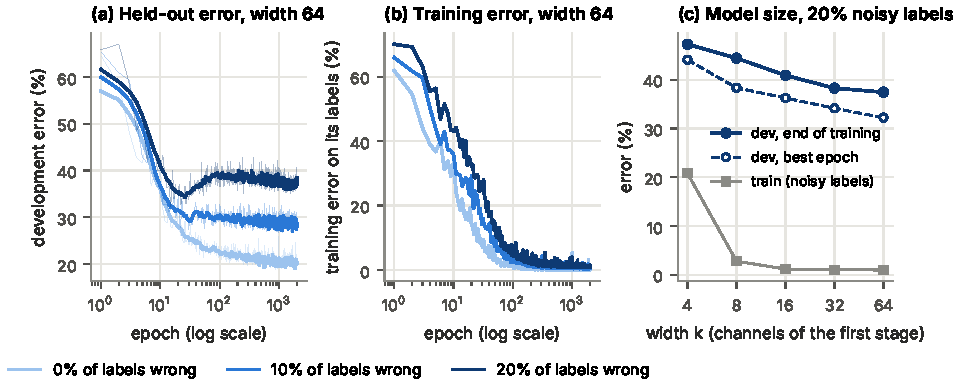
\includegraphics[width=\linewidth]{figs/fig_dd2000.pdf}
  \caption{\textbf{Up to 4{,}000 epochs of ResNet18 from scratch on $32\times32$ emoji}\rep. (a) Development error of the width-64 network for three levels of label noise (the 20\% run lasted 4{,}000 epochs, the others 2{,}000); thin lines are per epoch, thick lines a 9-epoch moving average. With 20\% wrong labels, error falls, rises while the noise is memorised (b) and descends again slowly, then levels off. (c) At 20\% noise, against width: error at the end of training (mean of the last 50 epochs) and at the best epoch, training error, and the error with half of the training images (triangles).}
  \label{fig:dd2000}
\end{figure}

\subsection{Did we overfit or underfit?}
\label{sec:fit}
A model underfits when it cannot even fit its training data (high bias: training and validation accuracy are both low and close), and overfits when it fits the training data much better than new data (high variance: a large and growing gap). \Cref{tab:fit} puts the training and validation numbers of every model whose curves we saved side by side. Training accuracy is measured on the fly during each epoch, with augmentation, dropout and stochastic depth active, so it slightly understates how well the network fits the clean training images.

\begin{table}[t]
\centering\small
\caption{\textbf{Training versus validation} at the checkpoint each run kept\ver. ConvNeXt values are the mean of the five folds at epoch 10 for a single model without test-time augmentation; the ensemble's out-of-fold accuracy is 97.69\%.}
\label{tab:fit}
\setlength{\tabcolsep}{4.5pt}
\begin{tabular}{@{}lrrrrrl@{}}
\toprule
Model (epoch kept) & Train acc. & Val.\ acc. & Gap & Train loss & Val.\ loss & Diagnosis\\
\midrule
Baseline CNN, 30 Sept.\ (20 of 20) & 74.96\% & 76.71\% & $-1.8$ & 0.722 & 0.714 & underfits\\
EmojiCNNv2 (23 of 25) & 93.82\% & 90.96\% & 2.9 & 0.194 & 0.309 & slight underfit\\
EmojiCNNv2 + metadata (25 of 25) & 96.24\% & 93.38\% & 2.9 & 0.133 & 0.240 & as above\\
ConvNeXt-Tiny, 5 folds (10 of 10) & 99.92\% & 97.62\% & 2.3 & 0.004 & 0.114 & benign fit\\
\bottomrule
\end{tabular}
\end{table}

\paragraph{The first CNN underfitted} Its training accuracy was 75\%, no higher than its validation accuracy, and both were still rising when training stopped after 20 epochs. That is the signature of high bias: the network, its optimiser and its training budget were too weak to fit the data at all, and more regularisation or more data would not have helped. We fixed it with capacity and optimisation (BatchNorm, a fourth stage, AdamW with OneCycle), not with more data, and gained 14 points.

\paragraph{EmojiCNNv2 is still slightly bias-limited} It fits 94\% of its training images and generalises to 91\%, a gap of about three points. The gap is small and stable over the last epochs (\cref{fig:descent}b), so variance is not the main problem; the remaining errors come from what a 0.39\,M-parameter network sees at 96\,px. A larger pretrained model at higher resolution removed most of them (+6.1 points on the same 1{,}979 validation images), which is what one expects when the limit is bias rather than variance.

\paragraph{The final ConvNeXt fits the training set, and that is benign} By the last epoch it classifies 99.9\% of its training images correctly with a training loss of 0.004, 27 times lower than its validation loss: in the classical sense it has memorised the training set. Yet its validation accuracy kept rising until epoch 9 and held at epoch 10, which is exactly why the last-epoch checkpoint beats the lowest-loss one (\cref{sec:epoch}). The overfitting shows in the probabilities, not in the decisions: the network becomes over-confident on the few images it gets wrong, which raises the validation loss while accuracy still improves. Four further checks point the same way. The private leaderboard score (0.98218) is above the out-of-fold estimate (97.69\%). The five folds agree within 0.4 points, the spread expected from sampling alone. Stronger regularisation (rotation and scaling augmentation with label smoothing, E7) lowered accuracy instead of raising it. And retraining on all the data, which would help a variance-limited model, changed the private score by only $+0.14$ and $-0.08$ points.

\paragraph{We did not overfit the validation set or the leaderboard} Every split groups exact duplicates, so no image is validated against a copy of itself; the final checkpoint rule (last epoch) involves no selection on validation data; the test set was never used to choose anything; and every model produced by the codebase scores higher on the private half of the test set than on our validation estimate (\cref{fig:kaggle}). If anything, our validation protocol is conservative.


\subsection{Error analysis and explainability}
\label{sec:errors}
The 228 out-of-fold errors are not spread evenly. Only 28 of them cross an export family: accuracy is \pct{96.6} inside the 72\,px family (\num{5906} images), \pct{99.7} in the 160\,px family (\num{1486}) and \pct{99.2} in the 240\,px family (\num{2487}) (\cref{fig:families}). The network never sees the native size, since every image is resampled to 224\,px, yet it separates the three families from the rendering alone and spends its errors on vendors that draw alike within a family. The smaller models show the trend: the September CNN made 176 cross-family errors, EmojiCNNv2 57, and the fusion model, which is told the family by the metadata, 6.

\begin{figure}[t]
  \centering
  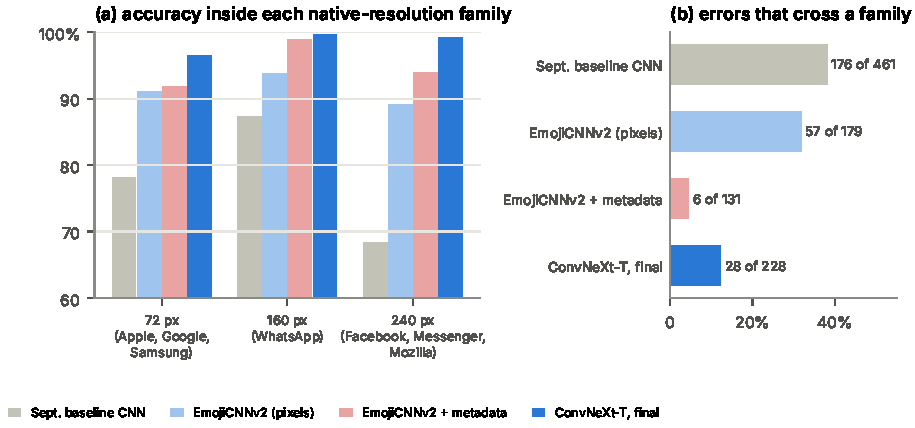
\includegraphics[width=\textwidth]{figs/fig10_families.pdf}
  \caption{\textbf{Errors stay inside an export family.} (a) Accuracy inside each native-resolution family; the three CPU models are scored on the stored split, the final model out-of-fold on all images. (b) Share of errors that assign an image to a vendor of another family. Only the fusion model, which receives the file format explicitly, crosses families less often than the final pixel-only model.}
  \label{fig:families}
\end{figure}

The confusion matrix (\cref{fig:confusion}) names the pairs: Apple predicted as Google 37 times, WhatsApp as Apple 36, Facebook as Apple 28, Google as Apple 17, Apple as Samsung 13 and Samsung as Apple 12. Apple sits at the centre for a documented reason: when WhatsApp released its own set in October 2017, Emojipedia described it as ``a unique set (albeit heavily inspired by the Apple Color Emoji font)'' \cite{emojipedia2017whatsapp}, and Apple, Google and Facebook share conventions for faces. \Cref{fig:failures} shows the most confident mistakes. Several are near-identical designs across related vendors; others are flags, symbols or simple shapes with almost no vendor-specific drawing; a few look to us like drawings of the vendor the model predicted, which may point to label noise that we cannot verify.

\begin{figure}[t]
  \centering
  \begin{minipage}[t]{0.47\textwidth}\vspace{0pt}
    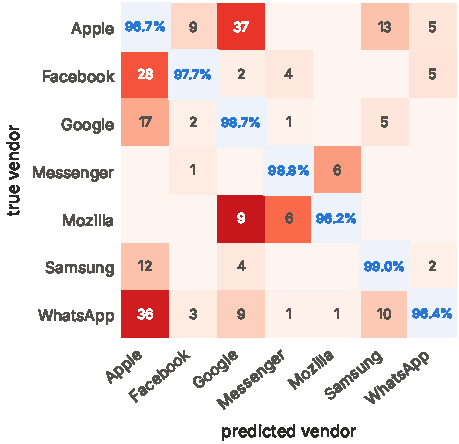
\includegraphics[width=\linewidth]{figs/fig9_confusion.pdf}
  \end{minipage}\hfill
  \begin{minipage}[t]{0.49\textwidth}\vspace{6pt}
    \caption{\textbf{Out-of-fold confusion matrix of the final model.} The diagonal gives per-vendor recall; off-diagonal cells give error counts, shaded by their share of the row. Apple is the hub of the confusions: WhatsApp's set was modelled on Apple's \cite{emojipedia2017whatsapp}, and Apple, Google and Samsung share the 72\,px export. Facebook, Messenger and Mozilla form the second cluster (240\,px), Messenger having used Facebook's set since October 2017 \cite{emojipedia2017messenger}.}
    \label{fig:confusion}
  \end{minipage}
\end{figure}

\begin{figure}[t]
  \centering
  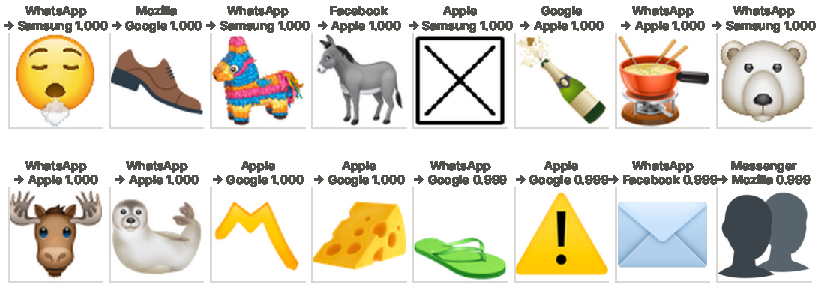
\includegraphics[width=\textwidth]{figs/fig12_failures.pdf}
  \caption{\textbf{The sixteen most confident out-of-fold mistakes} of the final model (true vendor $\to$ predicted vendor, confidence). Most are look-alike designs or images with little vendor-specific detail.}
  \label{fig:failures}
\end{figure}

To check what the networks attend to we applied Grad-CAM \cite{selvaraju2017gradcam} to the last convolutional stage of EmojiCNNv2 (\cref{fig:gradcam}). Its attention falls mostly on the drawing itself (outlines, eyes, shaded regions); on flat designs such as flags or a lozenge it spreads along the edge of the shape, where anti-aliasing differs between vendors. We see no case where it rests on the empty canvas, which is what the preprocessing was meant to ensure. The small model's confusions follow the same groups as the final model's: Facebook with Messenger, Mozilla with those two, Apple with Samsung (\cref{app:extra}).

\begin{figure}[t]
  \centering
  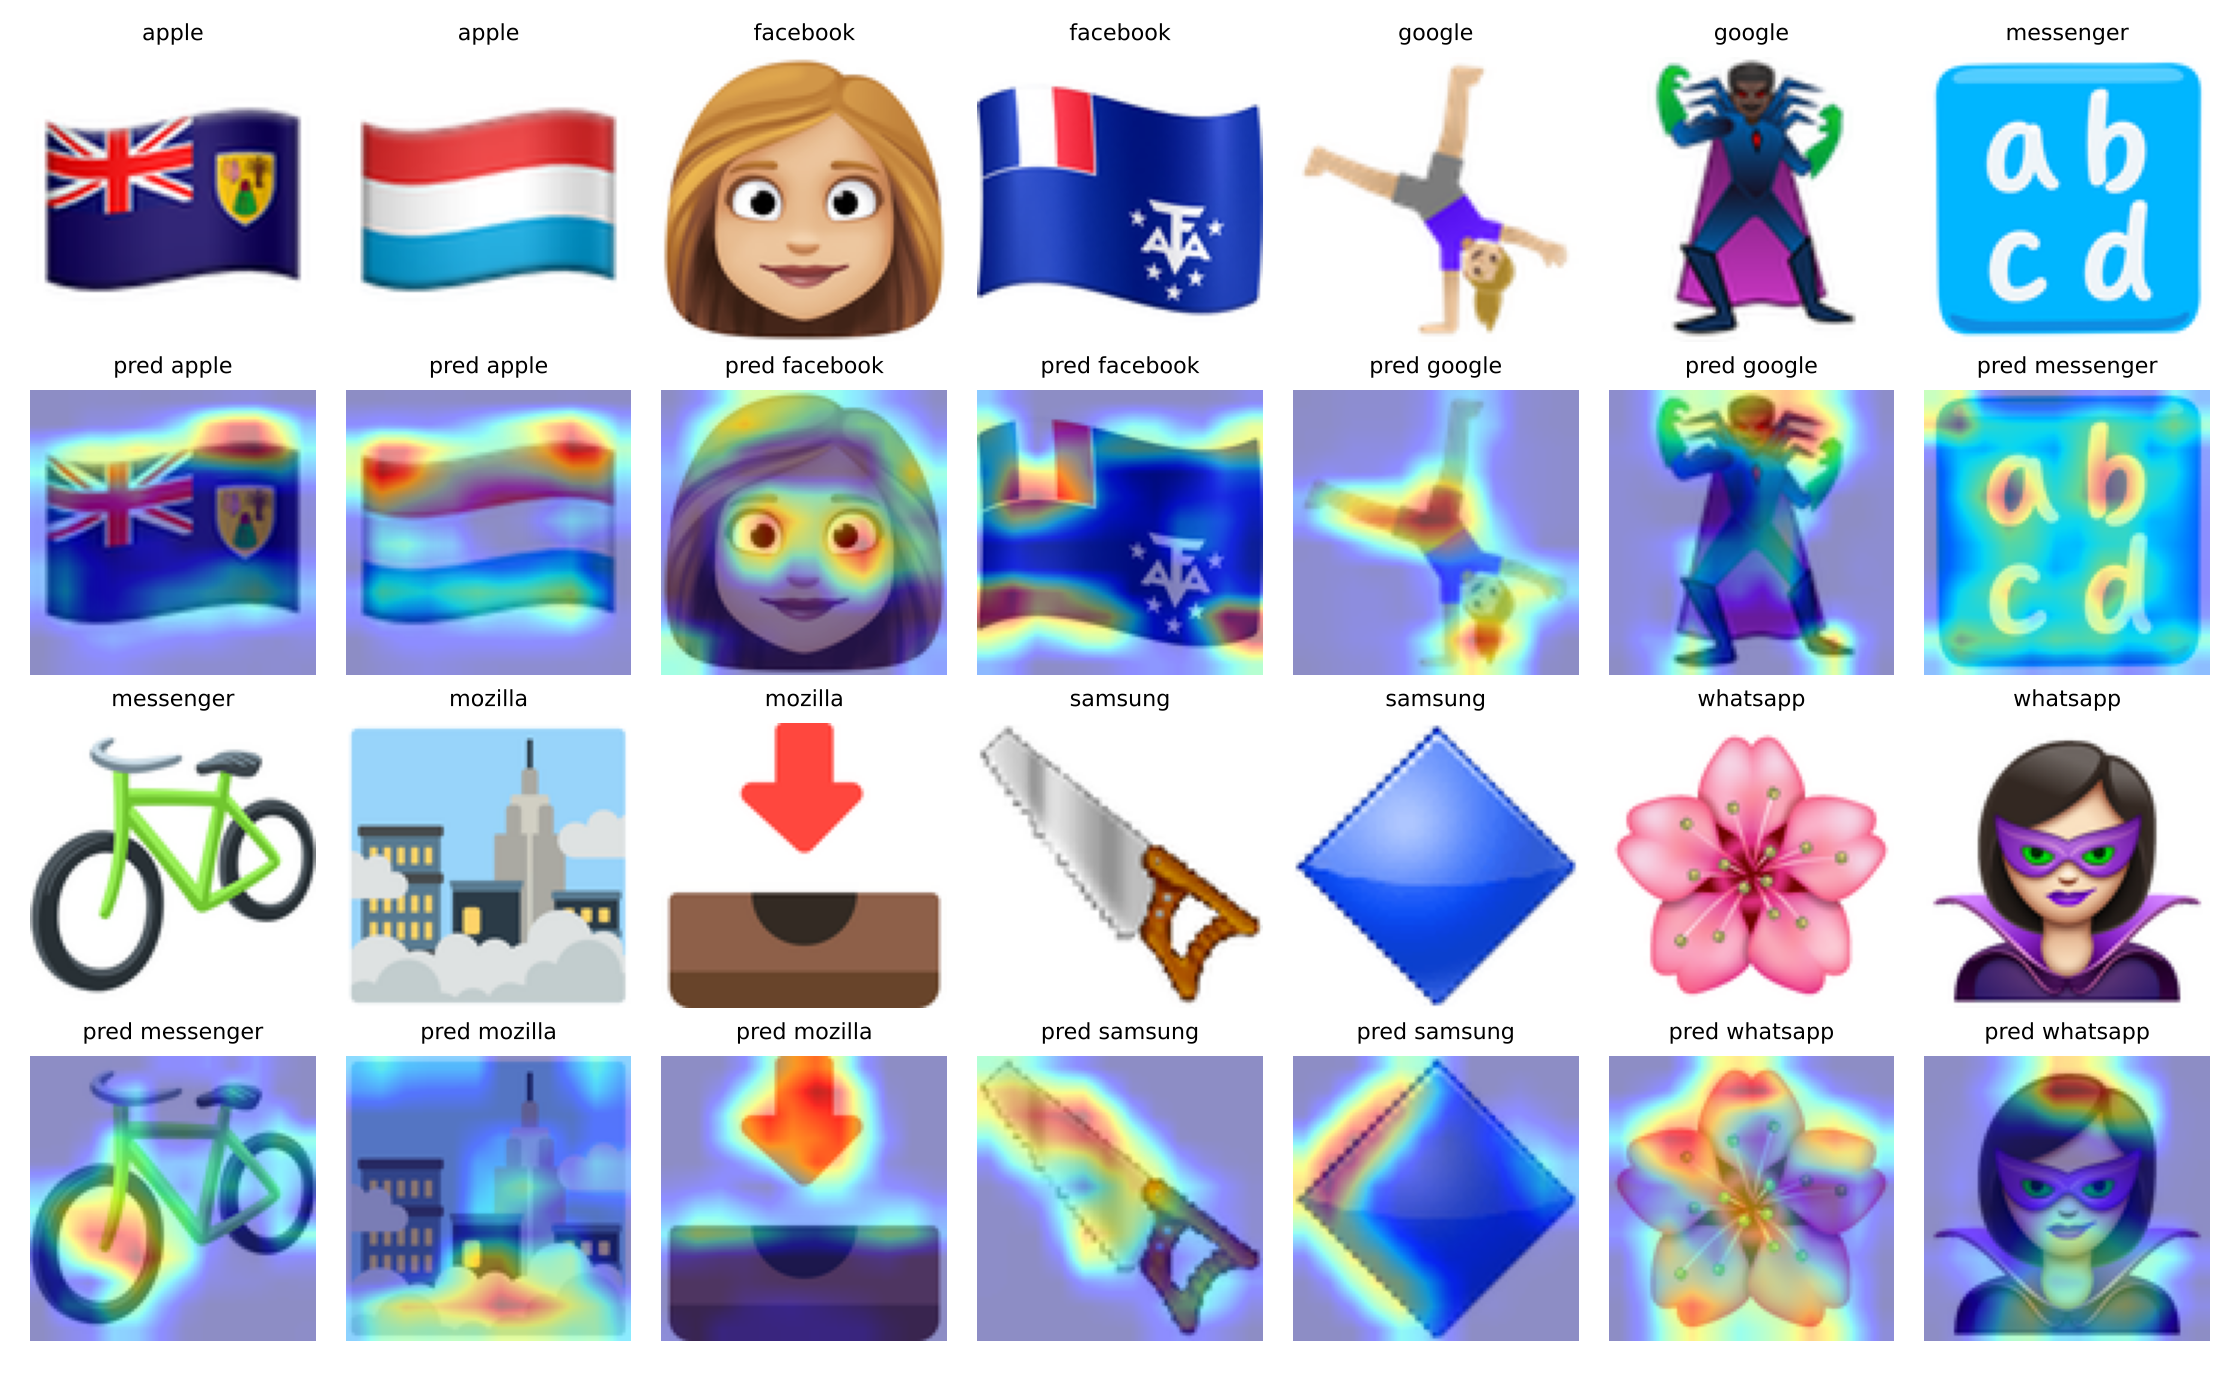
\includegraphics[width=0.74\textwidth]{figs/gradcam_emojicnnv2.png}
  \caption{\textbf{Grad-CAM on EmojiCNNv2} for correctly classified validation images, two per vendor. Top rows: input; bottom rows: Grad-CAM heat map of the predicted class. Attention concentrates on contours, eyes and shading, and on shape edges for flat designs.}
  \label{fig:gradcam}
\end{figure}

\subsection{Kaggle leaderboard}
\label{sec:kaggle}
The leaderboard splits the test set into a public half, shown during the competition, and a private half (about \pct{50} of the test images) that decides the final ranking. \Cref{tab:kaggle} lists the team's entries with both scores, read from the competition page after it closed. Every file produced by this codebase scores \emph{above} its validation estimate on the private half, by 0.5 to 2.2 points (\cref{fig:kaggle}). For the ConvNeXt files part of this is expected, because the out-of-fold estimate scores single fold-models while test predictions average five; for every model it means the protocol did not flatter us.

\begin{table}[t]
\centering\small
\caption{\textbf{Kaggle scores} (accuracy) of the team's entries, read on 27 October 2026 after the competition closed. Kaggle ranks a team by the better private score of its two selected entries ($\checkmark$). One early test entry (private 0.77874) and a duplicate upload are omitted. $^\S$On the DINOv2 branch's own 1{,}976-image development split, which was reused for earlier choices.}
\label{tab:kaggle}
\footnotesize\setlength{\tabcolsep}{4pt}
\begin{tabular}{@{}llrrrc@{}}
\toprule
Entry & Model & Val. & Public & Private & \\
\midrule
\rowcolor{panel}$\checkmark$ \code{convnext224\_last} & final model (run B), this paper & 97.69\% & 0.98319 & 0.98218 & \ver\\
\code{convnext224\_AB\_10models} & 10-checkpoint average (ablation) & 97.70\% & 0.98279 & 0.98198 & \ver\\
\code{emojicnnv2\_fusion} & EmojiCNNv2 + file metadata & 93.38\% & 0.93824 & 0.94615 & \ver\\
\code{emojicnnv2} & EmojiCNNv2, pixels only & 90.96\% & 0.90747 & 0.91700 & \ver\\
\code{adam\_baseline} & September baseline CNN & 76.71\% & 0.77546 & 0.78906 & \ver\\
\midrule
$\checkmark$ \code{E15\_ens\_full\_3models} & 3 ConvNeXt (224 bicubic, 144/216 nearest) & & 0.98117 & \textbf{0.98238} & \rep\\
\code{E13v\_ens\_val\_3models} & ensemble E8 + E12b + E13 & & 0.97772 & 0.97955 & \rep\\
\code{E9\_ens\_convnext128\_224} & ConvNeXt 128 + 224\,px & 97.93\% & 0.97671 & 0.97874 & \rep\\
\code{E10b\_convnext\_tiny\_224\_full} & E8 retrained on all data & & 0.97833 & 0.97773 & \rep\\
\code{E11\_ens\_full\_128\_224} & E9 retrained on all data & & 0.97914 & 0.97793 & \rep\\
\code{E8\_convnext\_tiny\_224} & ConvNeXt-Tiny 224\,px & 97.57\% & 0.97408 & 0.97631 & \rep\\
\code{submission2} (Lina) & frozen ResNet18 + hand-crafted, RBF SVM & 96.76\% & 0.96719 & 0.96983 & \rep\\
\code{submission} (Lina) & extra-trees, pixels + colour + alpha & 82.14\% & 0.81838 & 0.83259 & \rep\\
\code{dinov2\_convnext\_ensemble} & DINOv2 + ConvNeXt, partly tuned, 50:50 & 97.12\%$^\S$ & 0.96881 & 0.96477 & \rep\\
\code{submission} (Charles) & ResNet18, 160\,px + file format & 96.4\% & 0.95889 & 0.96396 & \rep\\
\code{dinov2\_finetuned} & DINOv2 ViT-S/14, last 2 blocks tuned & 95.90\%$^\S$ & 0.95586 & 0.95607 & \rep\\
\code{E3\_simple\_cnn\_white} & simple CNN, white compositing & 93.62\% & 0.93642 & 0.94331 & \rep\\
\bottomrule
\end{tabular}
\end{table}

\begin{figure}[t]
  \centering
  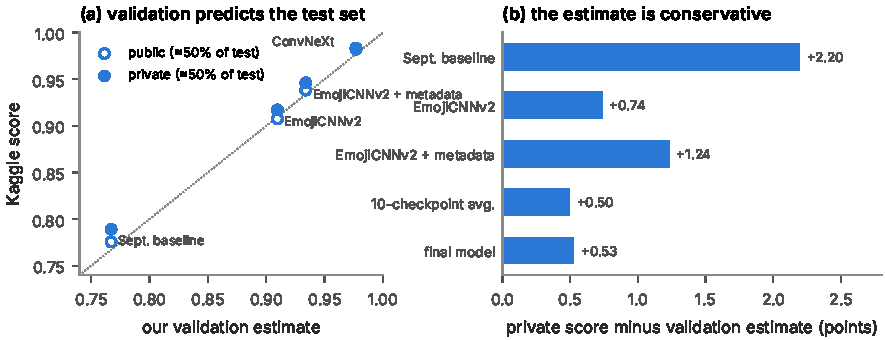
\includegraphics[width=\textwidth]{figs/fig11_kaggle.pdf}
  \caption{\textbf{Validation estimates against the hidden test set}, for the five files produced by the codebase. (a) Kaggle accuracy against our validation estimate; the dotted line is $y=x$. (b) Private score minus validation estimate: positive for every model, so the estimates are, if anything, conservative.}
  \label{fig:kaggle}
\end{figure}

The team's two selected entries at the close were our final model and Erdem's E15, a soft vote of three ConvNeXt-Tiny models trained on all training data, one at 224\,px with bicubic resizing and two at 144 and 216\,px with nearest-neighbour resizing, which are exact integer upscalings of the 72\,px files and follow the same exact-pixel logic as our augmentation. E15 scored 0.98238 on the private half, our final model 0.98218, a difference of about one image out of roughly \num{4940}. The team finished fifth of 18 teams on the private leaderboard, with the same score as the fourth-placed team. The two leading teams scored 0.99979 and 0.99919; we do not know their methods.

\subsection{What did not work}
\label{sec:nowork}
\begin{itemize}[leftmargin=1.2em]
  \item \textbf{Frozen ImageNet features with a linear head}: \pct{77.48}\rep, below a 0.4\,M-parameter CNN trained from scratch. With hand-crafted style descriptors and an RBF SVM on top, the same frozen features reached \pct{96.76}\rep.
  \item \textbf{Resampling augmentation and label smoothing}: minus 1.5 points on ConvNeXt-Tiny at 128\,px\rep. Three things changed at once (rotation and scaling, label smoothing, 15 instead of 10 epochs), so the run does not say which one hurt, but it agrees with the exact-pixel argument of \cref{sec:recipe}.
  \item \textbf{Voting with weaker members}: adding ResNet18 or the small CNN to the ConvNeXt ensemble lowered accuracy to 97.3 to \pct{97.4}\rep; a DINOv2 + ConvNeXt ensemble scored 0.96477 private against 0.98218 for our ConvNeXt alone (\cref{sec:dino}); learned fusion of three experts and two decision models never beat their plain average (\cref{sec:fusion}); and averaging in our own earlier snapshots did not help (\cref{sec:epoch}). Averaging helps between comparably strong models.
  \item \textbf{The September training budget}: constant Adam $10^{-3}$ for 20 epochs left the first CNN underfitting at \pct{75} training accuracy\ver; BatchNorm and OneCycle, not more parameters, closed most of the gap.
  \item \textbf{Keeping the lowest-validation-loss checkpoint}: 0.40 points below keeping the last epoch\ver.
\end{itemize}

% ================================================================== 6 AI AND CODE
\section{AI and code}
\label{sec:code}

\subsection{Codebase and reproducibility}
The submitted codebase is a small Python library (\code{src/emoji\_provider}: data, EDA, models, training, evaluation, metadata model, submission writer) with scripts and one notebook as entry point, built on PyTorch \cite{paszke2019pytorch}, \texttt{timm} \cite{wightman2019timm} and scikit-learn \cite{pedregosa2011sklearn}. \code{README.md} gives the exact commands of both GPU runs and of the Colab, Databricks and laptop variants; running it on a new machine needs only the Kaggle archive and the codebase zip. Every script checks its inputs with assertions (label columns, ID sets, train/test disjointness, duplicate isolation across splits, submission format and a round trip through CSV). Each run writes its configuration, device, kept epoch and package versions, its training history, its validation and test probabilities and its figures, so every number and figure in this paper is regenerated from saved outputs by \code{scripts/build\_report\_tables.py} without retraining; the full console log of both GPU runs is kept. Seeds are fixed, the validation split and the fold assignment are files, six unit tests pass, and a smoke mode exercises the whole GPU path on a laptop in minutes. The strongest reproducibility check was not planned: run B reproduced run A epoch by epoch to the last decimal.

\begin{center}\small
\begin{tcolorbox}[enhanced,colback=panel,colframe=panel,arc=2pt,boxrule=0pt,left=6pt,right=6pt,top=4pt,bottom=4pt,width=\textwidth]
\ttfamily\scriptsize
notebooks/Emoji\_Provider\_Classification.ipynb \hfill\textrm{\color{ink2}entry point (RunPod / Colab / Databricks / laptop)}\\
src/emoji\_provider/ \enspace data.py \; eda.py \; models.py \; train.py \; evaluate.py \; metadata\_model.py \; submit.py\\
scripts/ \enspace run\_cpu\_experiments.py \; train\_backbone.py \; make\_final\_submission.py \; build\_report\_tables.py\\
data/ \enspace split\_seed42.csv \; baseline\_sept30/best\_model.pt\\
outputs/ \enspace eda/ \; cpu/ \; convnext224/ (run A) \; convnext224\_last/ (run B) \; submissions/ \; runpod\_training\_logs.txt\\
README.md \; RUNBOOK.md \; AI\_USAGE.md \; requirements.txt \; requirements-gpu-runtime.txt \; tests/
\end{tcolorbox}
\end{center}

\subsection{Compute}
EmojiCNNv2 trains at 143\,s per epoch on two CPU cores (25 epochs). ConvNeXt-Tiny at 224\,px takes 2.4 to 2.9 minutes per fold, 13.0 minutes for the five folds, on an NVIDIA RTX 4090 rented on demand from RunPod at \$0.89 per hour; each run used about 16 minutes of pod time including PNG decoding, inference with test-time augmentation and figures, and both runs together cost about \$1.10. A single 224\,px model took about 2\,h\,10 on an Apple M4 laptop\rep. Package versions are listed in \cref{app:env}.

\subsection{Use of AI tools}
As the course allows, AI assistants were used for code and experiments, and, as the teacher allowed in class, for drafting this paper; every use and its prompts are listed in \code{AI\_USAGE.md}. The September baseline notebook was generated and debugged with OpenAI Codex. OpenAI's ChatGPT and Codex wrote and ran the DINOv2, style-feature, fusion and decision-model experiments of \cref{sec:dino,sec:fusion}. Claude (Anthropic) wrote the submitted codebase, ran the CPU experiments, drove the two GPU runs on a pod created by the team, generated the tables and figures from the saved outputs and drafted the text; the team chose the experiments, reviewed every claim against the outputs and is responsible for the content.

% ================================================================== 7 CONCLUSION
\section{Conclusion}
\label{sec:conclusion}
Recognising who drew an emoji is a style problem, and the project taught us as much about the data as about models. Looking at the files before the pixels exposed a shortcut worth \pct{87} accuracy without any drawn pixel; removing it made every later comparison about what the network sees. On the modelling side the lessons were plain. A small CNN trained properly beats hand-crafted features by ten points. Pretrained features help most once the whole backbone is fine-tuned; frozen, they need hand-crafted style descriptors and a non-linear classifier to compete. Input resolution mattered more than the architecture. Augmentations that resample the image erase the detail that identifies the vendor. And at \pct{97} accuracy the rule for choosing a checkpoint is worth 0.4 points: the last epoch of a OneCycle schedule is both the simplest and the best choice we found, because validation loss rewards hedging while accuracy rewards decisions. The final ConvNeXt-Tiny ensemble reaches \pct{97.69} out-of-fold and 0.98218 on the private leaderboard, separates the three export families from pixels alone, and fails on documented look-alikes, the behaviour of a model that learned style rather than file format.

\paragraph{Limitations} The reported rows of \cref{tab:ladder} come from single runs on a different split and carry no error bars. Our architecture comparison rests on those runs. We did not train at the native 240\,px, did not retrain the final recipe on all training data, and could not verify the labels of the most confident errors.

\paragraph{Future work} Train at native resolution with integer (nearest-neighbour) upscaling of the 72\,px files: in Erdem's controlled test the resize filter mattered at 144\,px (+0.9 points) but not at 216\,px, and the 72\,px files stayed the main source of error, so a model built around their native grid is the open question; try a two-stage classifier that predicts the export family and then the vendor within it, an explicit version of what the network does implicitly; run a seed study to put error bars on the architecture comparison; and fine-tune DINOv2 (or DINOv3, once its weights are available) end to end, to separate the effect of the architecture from that of the partial fine-tuning. Combining backbones is worth it only with an expert whose mistakes differ from theirs: with hand-crafted style features, the fusion transformer and two decision models all fell short of a plain average, while with the file-byte model a parameter-free geometric mean or a most-confident-expert rule gained up to 0.9 points (\cref{sec:fusion}); the decision model Jev never beat the simple rules. Training much longer is not: on clean labels the curves have no second descent to wait for (\cref{sec:descent}).

% ================================================================== REFERENCES
\FloatBarrier
\small
\bibliographystyle{unsrtnat}
\bibliography{refs}
\normalsize

% ================================================================== APPENDIX
\appendix
\section{Erdem's experiment log (13 to 14 October)}
\label{app:log}
\label{app:log}
\begin{table}[H]
\centering\small
\caption{Erdem's experiment series on a stratified 80/20 split (seed 42)\rep. Public scores where the experiment was submitted. Code, commands, per-run records and saved probabilities: \texttt{members/erdem-sanver/}.}
\begin{tabularx}{\textwidth}{@{}l>{\raggedright\arraybackslash}Xrr@{}}
\toprule
Id & Model and method & Val.\ acc. & Public\\
\midrule
E1a & random forest on file metadata (size, mode, hidden colour) & 65.84\% & \\
E1b & RBF SVM on 512-bin colour histogram + HOG, 64\,px & 81.28\% & \\
E2 & simple CNN (32-64-128), naive RGB load, 96\,px & 92.11\% & \\
E3 & same CNN, alpha-composited on white & 93.62\% & 0.93642\\
E4 & ResNet18, frozen ImageNet features, 128\,px & 77.48\% & \\
E5 & ResNet18, fine-tuned, 128\,px & 93.72\% & \\
E6 & EfficientNet-B0, fine-tuned, 128\,px & 93.12\% & \\
E6b & ConvNeXt-Tiny, fine-tuned, 128\,px & 95.90\% & \\
E7 & as E6b + rotation/scale augmentation + label smoothing & 94.38\% & \\
E8 & ConvNeXt-Tiny, fine-tuned, 224\,px & 97.57\% & 0.97408\\
E9 & soft vote E6b + E8 & 97.93\% & 0.97671\\
E10a, E10b & E6b, E8 retrained on all data (no validation score); E10b submitted & & 0.97833\\
E11 & soft vote E10a + E10b & & 0.97914\\
E12a & ConvNeXt-Tiny, 144\,px, bicubic resize (control for E12b) & 96.31\% & \\
E12b & ConvNeXt-Tiny, 144\,px, nearest-neighbour resize & 97.22\% & \\
E13 & ConvNeXt-Tiny, 216\,px, nearest-neighbour resize & 97.47\% & \\
E13v & soft vote E8 + E12b + E13 & 98.13\% & 0.97772\\
E14a, E14b & E12b, E13 retrained on all data (no validation score) & & \\
E15 & soft vote E10b + E14a + E14b & & 0.98117\\
E16 & E12b + \num{9046} pseudo-labelled test images (E13v confidence $\geq 0.99$) & 97.72\% & \\
\bottomrule
\end{tabularx}
\end{table}

\section{Who tried what}
\label{app:who}
\begin{table}[H]
\centering\small
\caption{Methods tried by each team member, with their best recorded score. The repository has one folder per member (\texttt{members/}) that holds these notes and, where available, the code.}
\begin{tabularx}{\textwidth}{@{}l>{\raggedright\arraybackslash}X>{\raggedright\arraybackslash}p{40mm}@{}}
\toprule
Member & Methods & Best recorded score\\
\midrule
Adam Zeraiki & First CNN (30 September, with OpenAI Codex); EmojiCNNv2 and the metadata diagnostic; ConvNeXt-Tiny 5-fold runs A and B and the 10-checkpoint average; DINOv2 + ConvNeXt combination; this paper & 97.69\% OOF, 0.98218 private (final model)\\
Erdem Sanver & Experiments E1a to E15: metadata random forest, HOG + colour SVM, simple CNN with and without compositing, ResNet18 frozen and fine-tuned, EfficientNet-B0, ConvNeXt-Tiny at 128 and 224\,px, augmentation study, ensembles, retraining on all data, nearest-neighbour upscaling & 97.93\% validation (E9); 0.98238 private (E15, team best)\\
Lina Oumhand & DINOv2 fine-tuned; two earlier entries (no description recorded) & 0.96983 private (\texttt{submission2})\\
Charles Montluc & ResNet18 pretrained on ImageNet, fine-tuned on 160\,px RGB images & 0.96396 private\\
\bottomrule
\end{tabularx}
\end{table}


\section{Per-vendor results of the CPU models}
\label{app:extra}
\begin{table}[H]
\centering\small
\caption{Recall per vendor on the stored \num{1979}-image split\ver.}
\footnotesize\setlength{\tabcolsep}{4pt}
\begin{tabular}{@{}lrrrrrrrr@{}}
\toprule
Model & Apple & Facebook & Google & Messenger & Mozilla & Samsung & WhatsApp & Macro F1\\
\midrule
September baseline & 0.765 & 0.693 & 0.940 & 0.421 & 0.744 & 0.751 & 0.817 & 0.738\\
EmojiCNNv2 & 0.897 & 0.834 & 0.964 & 0.917 & 0.878 & 0.972 & 0.881 & 0.907\\
EmojiCNNv2 + metadata & 0.920 & 0.910 & 0.953 & 0.926 & 0.841 & 0.986 & 0.922 & 0.926\\
\bottomrule
\end{tabular}
\end{table}

\section{Environment}
\label{app:env}
CPU experiments: Python 3.13, torch 2.14.1, torchvision 0.29.1, timm 1.0.30, scikit-learn 1.9.1, numpy 2.5.3, pandas 3.0.5, Pillow 12.3.0 (pinned in \code{requirements.txt}). GPU runs: RunPod PyTorch 2.8.0 image, torch 2.8.0+cu128, NVIDIA driver 570.169, RTX 4090 24\,GB, with scikit-learn and timm installed from PyPI on 17 October 2026. The September baseline was trained with torch 2.11.0+cu128; re-scored with the current versions it reproduced \num{1518} / \num{1979} correct exactly.

\end{document}
